\newpage
\section{Protocolli tra entità attive del sistema}
Seguendo il modello IDM un parametro importante da considerare per l'avanzamento delle entità passive è la distanza tra l'entità stessa e la fine della traiettoria del mezzo che si trova davanti o che l'entità potrebbe trovarsi davanti a seguito di uscite da ingressi o cambi corsia di altri mezzi che si trovano davanti al mezzo interessato. Tutta la logica dell'avanzamento viene quindi basata sul calcolo delle distanze ai mezzi seguenti il mezzo interessato. Il calcolo di questa distanza deve essere fatto in relazione alla posizione del mezzo che copriva nel quanto di tempo antecedente al quanto di tempo in cui viene effettuato l'aggiornamento della nuova posizione (anche per questo motivo il $\Delta$ del sistema non può assumere valori troppo grandi). Ribadendo quali sono le entità attive del sistema: incroci, strade principali, strade d'ingresso è necessario stabilire dei protocolli di comunicazione tra le entità. In particolare conviene dapprima fissare un ordine di esecuzione per le entità attive:

\begin{figure}[H] % Example image
\center{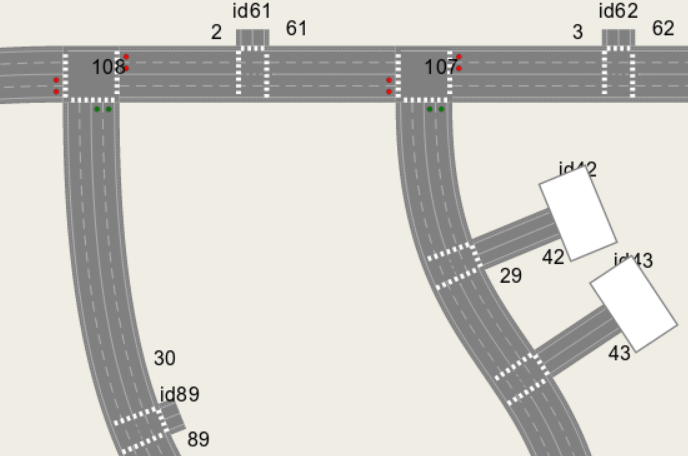
\includegraphics[width=0.9\linewidth]{EsempioMappa}}
\caption{Un frammento di mappa di un quartiere.}
\label{fig:Un frammento di mappa di un quartiere}
\end{figure}

Come da esempio in \ref{fig:Un frammento di mappa di un quartiere} si può notare che una strada principale è limitata al più da 2 incroci e una strada può o meno avere degli ingressi. Considerando questo modello conviene stabilire una dipendenza tra le seguenti entità attive: tra le strade principali e gli incroci; tra gli ingressi e le strade principali. \\
Un'entità attiva di tipo strada principale può iniziare a calcolare gli aggiornamenti di posizione delle entità passive solo dopo che gli incroci da cui è limitata hanno eseguito lo spostamento delle loro entità; questa dipendenza porta al seguente vantaggio: quando una strada principale deve eseguire l'avanzamento delle entità al $\Delta$ di sistema conosce lo stato aggiornato delle entità nell'incrocio e inoltre un incrocio potrà operare in un certo quanto di tempo conoscendo tutte le entità che dovranno essere spostate, dato che il task della strada principale non potrà demandare all'incrocio la gestione dello spostamento di una nuova entità se non dal quanto di tempo successivo. Analogamente, il vantaggio che si ricava nel far eseguire gli spostamenti delle entità ai task strade principali prima dei task strade d'ingresso è dovuto al fatto che un'entità strada d'ingresso potrà conoscere lo stato aggiornato della strada principale, inoltre questa dipendenza fa si che un task strada d'ingresso non potrà inserire nuove entità nelle strutture dati della strada principale in momenti non deterministici. Le dipendenze inserite, quindi, facilitano il controllo del passaggio di entità passive tra un gestore e l'altro (cioè tra un'entità attiva e l'altra), infatti le dipendenze sopra esposte fanno si che un task al ritorno dall'attesa conoscerà tutte le entità che sono in transizione tra i gestori interessati e non potranno presentarsene di altre fino al quanto di sistema successivo.

\subsection{Protocollo di avanzamento e aggiornamento dello stato delle entità}
In questa sezione viene esposta e analizzata la struttura di un'entità attiva. Innanzitutto occorre predisporre una "mailbox" per ogni entità attiva. Una mailbox è una entità reattiva di tipo risorsa che ha il compito di contenere lo stato delle entità che la rispettiva entità attiva ha in gestione; attraverso la mailbox le entità attive possono comunicare tra loro notificando inserimenti e/o rimozioni di entità da spostare, informando altre entità attive delle posizioni occupate dalle entità passive, dello stato della risorsa stessa ad esempio nel caso di incroci la risorsa dovrà rendere disponibile un'interfaccia per comunicare se il semaforo è verde o rosso, ecc.

\begin{codiceada}[caption={Template-Code entità attiva}, label=template-code]
loop
	synchronization_with_delta;
	mailbox.update_entity_status;	
	update_view;	
	move_entity;
end loop;
\end{codiceada}
\\
Dove:
\begin{itemize}
\item \textit{synchronization\_with\_delta} è la procedura utilizzata per permettere all'entità di entrare in sincronizzazione con il sistema al quanto di tempo successivo;
\item \textit{mailbox.update\_entity\_status} è la procedura utilizzata per aggiornare la posizione delle entità calcolate al quanto di tempo precedente; \item \textit{update\_view} è la procedura utilizzata per inviare al web server le posizioni delle entità aggiornate al nuovo delta;
\item \textit{move\_entity} è la procedura utilizzata per spostare le enitità in gestione all'entità attiva corrente.
\end{itemize}

A seconda poi del tipo di entità occorrerà eseguire delle attese per favorire la gestione delle precedenze e per facilitare la consistenza dello stato della risorsa in un preciso quanto di tempo. \\
Quindi a seconda del tipo di entità attiva sarà necessario integrare al template di codice in \ref{template-code} le seguenti strutture:
\begin{itemize}
\item per gli incroci:\\
\begin{codiceada}[caption={Template-Code incroci}, label=template-code-incroci]
loop
	-- same code rows: [2-5]
	wake_up_strade_principali;
	move_entity;
end loop;
\end{codiceada}
\\
Dove:
\begin{itemize}
\item \textit{wake\_up\_strade\_principali} è la procedura utilizzata per comunicare ad ogni strada principale interessata nell'incrocio che l'incrocio ha terminato l'aggiornamento delle entità per il quanto di tempo del sistema.
\end{itemize}
\item per le strade principali:\\
\begin{codiceada}[caption={Template-Code strade principali}, label=template-code-principali]
loop
	-- same code rows: [2-4]
	mailbox.wait_incroci;	
	move_entity;
	mailbox.finish_delta_updated;
end loop;
\end{codiceada}
\\
Dove:
\begin{itemize}
\item \textit{mailbox.wait\_incroci} è la procedura utilizzata dalla strada prinicipale per aspettare la terminazione dell'aggiornamento delle entità degli incroci interessati relativamente al quanto di tempo del sistema.
\end{itemize}
\item per le strade d'ingresso:\\
\begin{codiceada}[caption={Template-Code strade ingresso}, label=template-code-ingresso]
loop
	-- same code rows: [2-4]
	mailbox_urbana.wait_urbana_finish_delta;	
	move_entity;
end loop;
\end{codiceada}
\\
Dove:
\begin{itemize}
\item \textit{mailbox\_urbana.wait\_urbana\_finish\_delta	
} è la procedura utilizzata dalla strada d'ingresso per aspettare la terminazione dell'aggiornamento delle entità della strada principale alla quale l'ingresso si riferisce relativamente al quanto di tempo del sistema. Vale la pena qui dire che una strada d'ingresso apparterrà sempre allo stesso quartiere al quale appartiene la strada principale alla quale l'ingresso si riferisce.
\end{itemize}
\end{itemize}

\subsubsection{Gestione dello spostamento delle entità per le strade d'ingresso}
Vista la struttura disposta da un task di tipo strada ingresso, vedi \ref{template-code-ingresso}, qui in questa sezione viene analizzata la modalità dello spostamento delle entità passive da parte di un'entità di tipo ingresso.\\
Nel modello della mappa ciò che viene classificato come strada d'ingresso dispone di una corsia per senso di marcia, un marciapiede e una pista ciclabile.\\
Quindi di seguito viene riportato il sistema che si occupa dello spostamento delle entità degli ingressi e il protocollo di interazione con la strada principale alla quale l'ingresso si riferisce:
\begin{enumerate}
\item per questa tipologia di entità attiva possono essere spostati indifferentemente mezzi, bici o pedoni senza un ordine prioritario;
\item un'entità passiva viene inserita nel sistema attraverso le strade d'ingresso; occorre controllare se nella mailbox dell'ingresso sono state inserite delle entità per cui occorre iniziare lo spostamento; se vi sono delle entità occorre trasferirle dalla lista temporanea della mailbox alla lista che si occupa della gestione dello spostamento delle entità. La lista temporanea è necessaria dato che l'inserimento di nuove entità nella mailbox può avvenire in qualunque momento; sarà poi il task a decidere il momento per iniziare a spostare le nuove entità;
\item la strada d'ingresso può essere percorsa secondo il verso d'uscita della strada, oppure secondo il verso d'entrata della strada; considerando entrambi i versi di percorrenza l'ordine con cui le entità possono essere spostate può essere eseguito sia, dall'entità più vicina alla fine del verso di percorrenza all'entità inserita a inizio del verso di percorrenza, che viceversa; supponiamo che venga scelto l'ordine dall'entità più distante dalla fine del verso di percorrenza all'entità più vicina alla fine del verso di percorrenza;
\item un'entità passiva, seguendo il suo verso di percorrenza, può essere preceduta da un'altra entità passiva oppure semplicemente dalla sola limitazione della fine della strada d'ingresso;
\item se l'entità passiva (V\_A) presenta un'altra entità ad una posizione maggiore rispetto a V\_A stesso, rispetto al loro verso di percorrenza, allora il calcolo della distanza dall'entità precedente sarà una conoscenza disponibile localmente nella mailbox della strada d'ingresso; mentre se l'entità passiva non è preceduta da nessuna altra entità occorrerà controllare la posizione delle entità in uscita dagli ingressi (in gestione quindi al task delle strade principali) per le entità che seguono il verso di percorrenza in uscita dagli ingressi; mentre seguendo il verso di percorrenza in entrata dagli ingressi non ha alcuna importanza imporre un limite dato che l'entità ha concluso il percorso ed è in procinto di uscire dal sistema.
Per controllare la posizione delle entità in uscita dagli ingressi, il task potrà controllare l'avanzamento delle entità "cedute" alla strada principale direttamente dalla propria mailbox; infatti il protocollo di comunicazione tra task della strada principale e task ingresso prevede che il task della strada principale aggiorni le mailbox degli ingressi in merito all'avanzamento delle entità in uscita dagli ingressi fintanto che le entità interessate non siano uscite completamente dall'ingresso considerando la lunghezza dell'entità stessa;
\item per le entità che seguono il verso di percorrenza in uscita dagli ingressi occorre considerare se la loro posizione raggiunge la lunghezza dell'ingresso con l'aggiornamento della posizione alla fine del quanto del sistema in corso d'opera. Se l'entità alla fine del quanto, quindi dopo l'aggiornamento della nuova posizione raggiunge la fine della lunghezza dell'ingresso sarà necessario aggiungere l'entità nella mailbox della strada principale; questa operazione viene effettuata prima della nuova sincronizzazione da parte del task ingresso stesso, affinchè la strada principale quando rieffettua la sincronizzazione, che sarà dopo l'esecuzione delle operazioni degli ingressi, troverà nella mailbox la nuova entità da spostare e la troverà in posizione 0 nella traiettoria che dovrà intraprendere (gestita dalla strada principale); l'ingresso quindi rimuoverà l'entità che ha raggiunto la fine della strada d'ingresso dato che questa entità è stata inserita nella mailbox della strada principale e quindi dal prossimo quanto sarà in gestione dal task della strada principale interessata. La traiettoria che l'entità dovrà intraprendere deve essere calcolata dall'ingresso stesso, al fine di permettere alla strada principale di trovare un'entità da spostare correttamente configurata; il calcolo della traiettoria da intraprendere deve avvenire interrogando il servizio di locazione delle entità, disponibile in ogni quartiere. Tale servizio contiene tutti i percorsi e la storia del percorso eseguito di tutte le entità istanziate nel quartiere stesso. Un'entità quindi prima di essere inserita nella mailbox degli ingressi presenta già il percorso completamente configurato presso il gestore del servizio di locazione delle entità del quartiere. Il calcolo della traiettoria da intraprendere si basa sulle convenzioni utilizzate per la creazione della mappa;
\item il task ingresso dovrà infine eseguire lo spostamento delle entità passive che sono in transizione dalla strada principale all'ingresso stesso; il task della strada principale, per il quanto di sistema in corso, avrà già calcolato la nuova posizione dell'entità che è in procinto di entrare nella strada d'ingresso interrogando la mailbox dell'ingresso stesso al fine di apprendere la distanza della prima entità presente nell'ingresso secondo il verso che porta l'entità, dalla strada principale alla fine dell'ingresso; il task ingresso quindi dispone di un'entità che al $\Delta$ di sistema corrente non necessita il calcolo dell'avanzamento dato che è stato eseguito per conto del task della strada principale; utilizzando quindi una struttura temporanea per memorizzare queste entità in transizione sarà sufficiente per il task ingresso spostare, prima della nuova sincronizzazione, le entità dalla struttura temporanea alla struttura adibita per lo spostamento delle entità. Dopo la nuova sincronizzazione sarà l'ingresso stesso il responsabile della gestione delle entità che erano al $\Delta$ precedente in gestione dal task della strada principale.
\end{enumerate}
Il protocollo di avanzamento delle entità per gli ingressi prevede un ordine FIFO nell'avanzamento delle entità senza prevedere possibilità di sorpassi o attraversamenti pedonali; se l'entità è un veicolo allora questo potrà essere preceduto solamente dalla fine della strada o da un veicolo dello stesso tipo; analogamente per le entità di tipo pedone e bici.
\subsubsection*{Operazioni dopo la nuova sincronizzazione} 
Il task gestore della strada d'ingresso dopo aver effettuato l'operazione di risincronizzazione, potrà rendere effettivi gli aggiornamenti di posizione delle entità calcolati nel quanto di sistema precedente; l'operazione di aggiornamento per entità passive gestite da un'entità di tipo ingresso consiste semplicemente nel rendere effettivi gli aggiornamenti di posizione calcolati al quanto precedente. Quindi qui potrà essere notificata la view della nuova posizione delle entità che occupano alla fine del quanto di sistema precedente.  
\subsubsection{Gestione dello spostamento delle entità per le strade principali}
Dato il template per un task di tipo strada principale, vedi \ref{template-code-principali}, occorre stabilire le regole per poter effettuare lo spostamento delle entità attive per un task di questa tipologia.\\
Un'entità attiva di tipo strada principale ha la gestione degli spostamenti delle entità che devono essere spostate da o verso un ingresso. \\ Il task della strada principale dovrà gesitre lo spostamento di entità passive nelle traiettorie riportate nelle figure sottostanti:

\begin{figure}[H] % Example image
\center{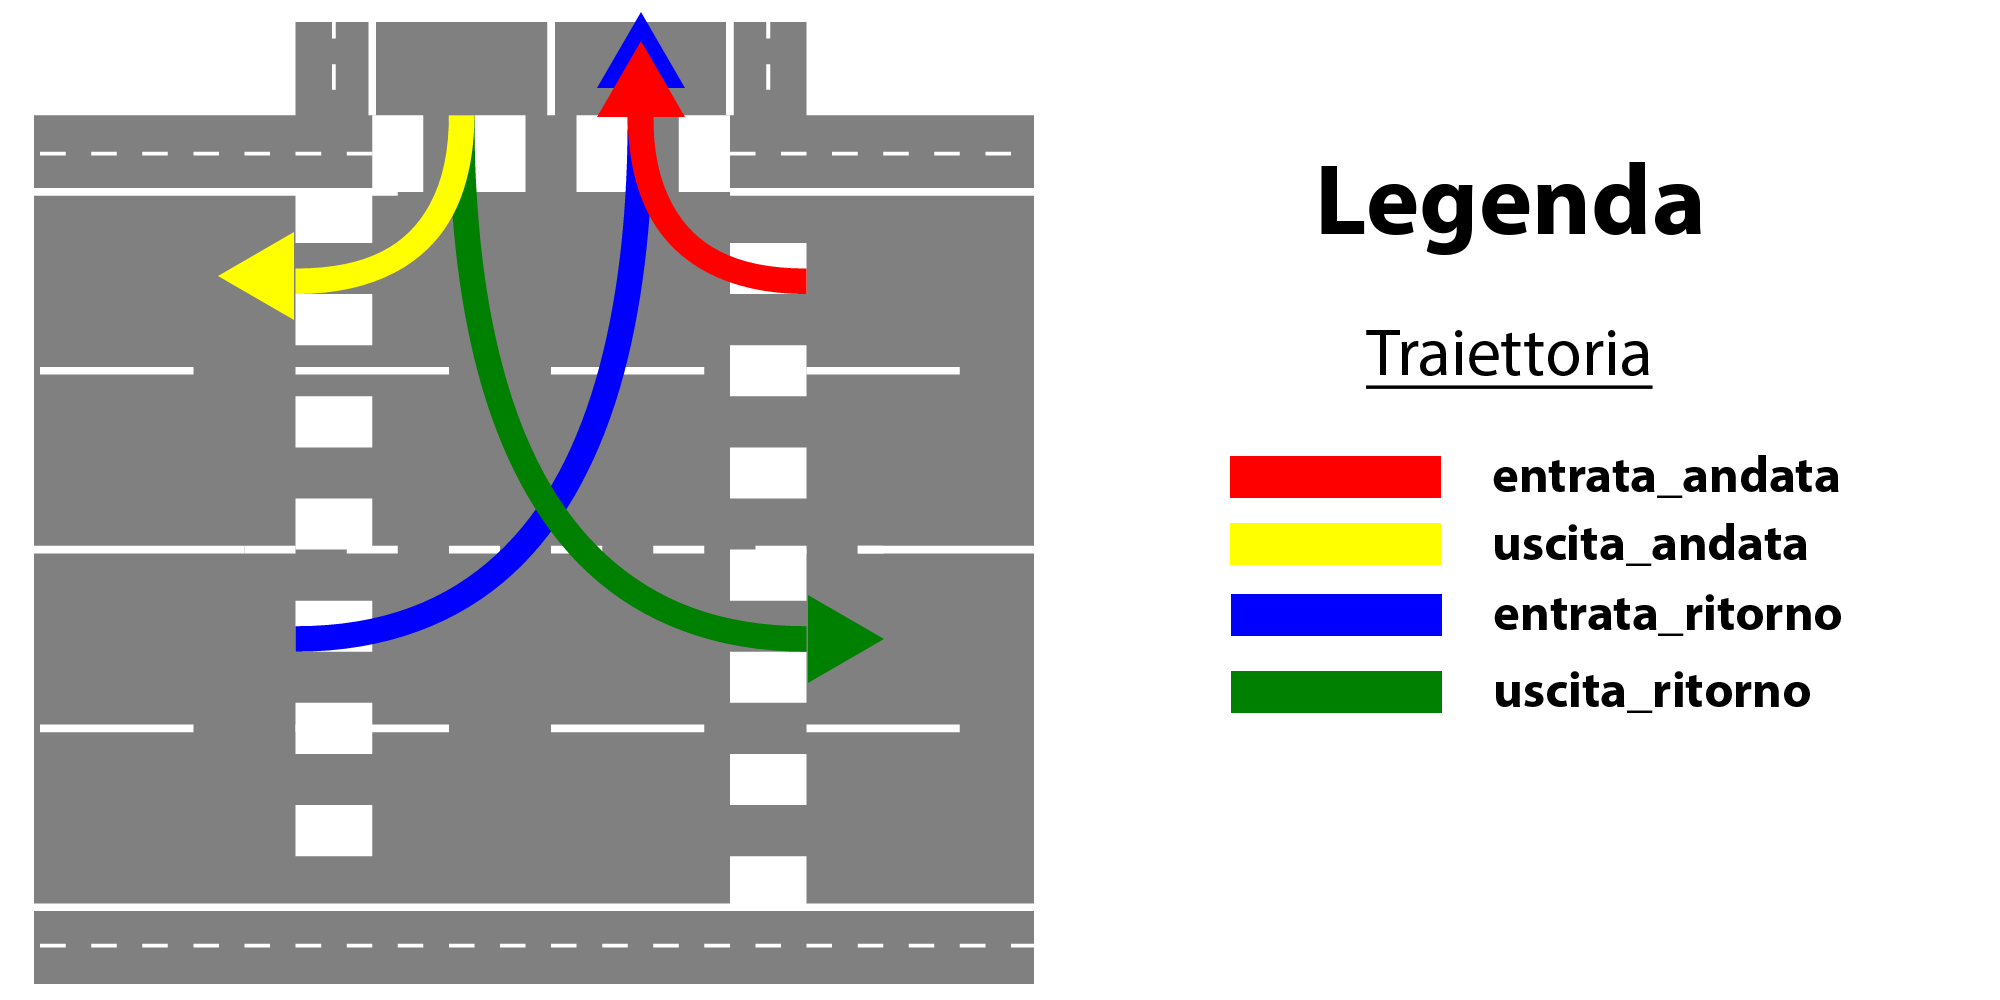
\includegraphics[width=1.0\linewidth]{traiettorie_ingresso_auto}}
\caption{Traiettorie in entrata/uscita ingresso per i veicoli.}
\label{fig:Traiettorie in entrata/uscita ingresso per i veicoli}
\end{figure}

\begin{figure}[H] % Example image
\center{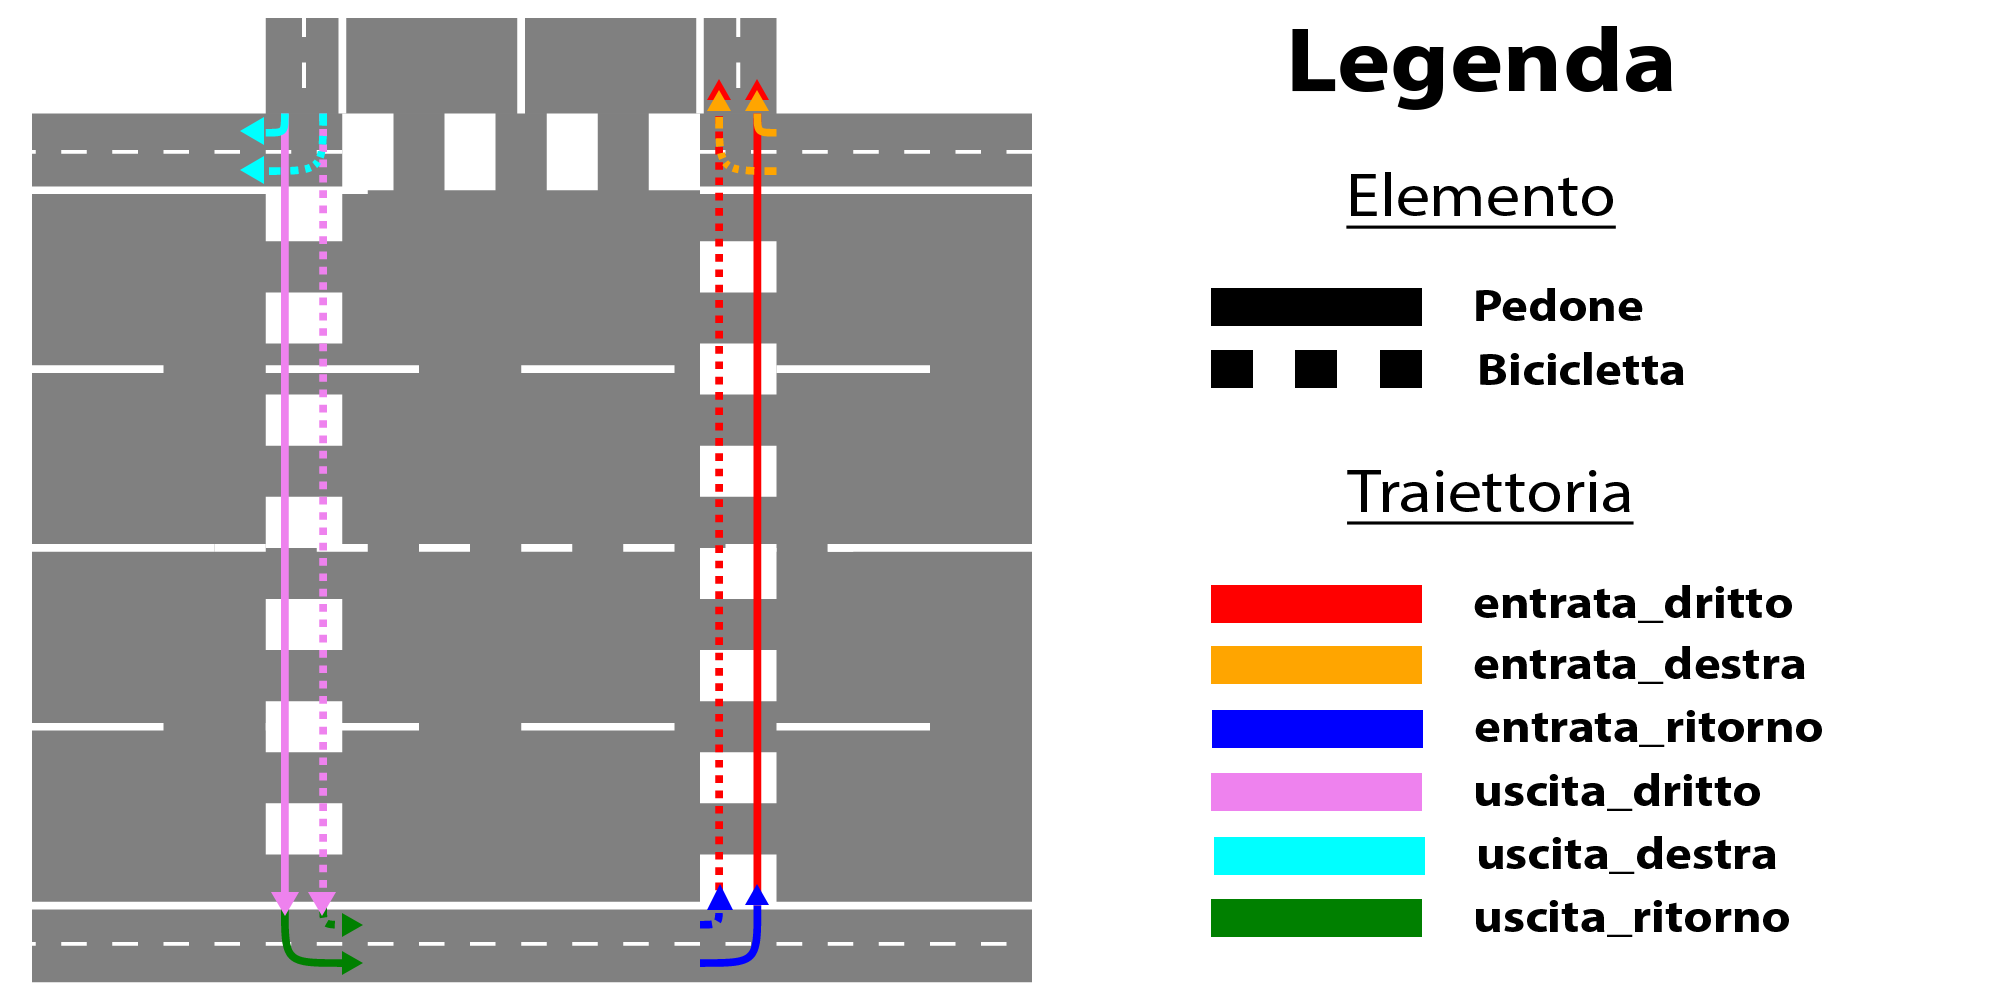
\includegraphics[width=1.0\linewidth]{traiettorie_ingresso_pedoni}}
\caption{Traiettorie in entrata/uscita ingresso per bici e pedoni.}
\label{fig:Traiettorie in entrata/uscita ingresso per bici e pedoni}
\end{figure}

Di seguito viene riportato il sistema responsabile della gestione dello spostamento delle entità e quindi il protocollo con cui l'entità attiva comunica con le entità attive di tipo incrocio. 
\begin{enumerate}
\item per un task di tipo strada principale occorre stabilire un ordine prioritario per le entità passive da spostare; dapprima si devono spostare le entità presenti su marciapiedi, su piste ciclabili e su strada, poi si devono spostare le entità presenti nelle traiettorie degli ingressi in gestione ai task delle strade principali di pedoni, bici e degli altri veicoli. 
Quest'ordine prioritario degli spostamenti è dovuto al fatto che gli spostamenti sulle traiettorie degli ingressi sono soggette a un sistema di precedenze non regolamentato da semafori, quindi devono essere stabilite le condizioni per abilitare o meno gli spostamenti nelle traiettorie in entrata e uscita dagli ingressi, in relazione alle posizioni delle entità su marciapiedi, piste ciclabili e strade calcolate in precedenza perchè a maggior priorità;
\item per lo spostamento di bici e pedoni rispettivamente sulla pista ciclabile e sul marciapiede occorre eseguire la seguente procedura:
\begin{enumerate}
\item un marciapiede/pista ciclabile può essere percorso seguendo un solo verso, di seguito un disegno specificativo:

\begin{figure}[H] % Example image
\center{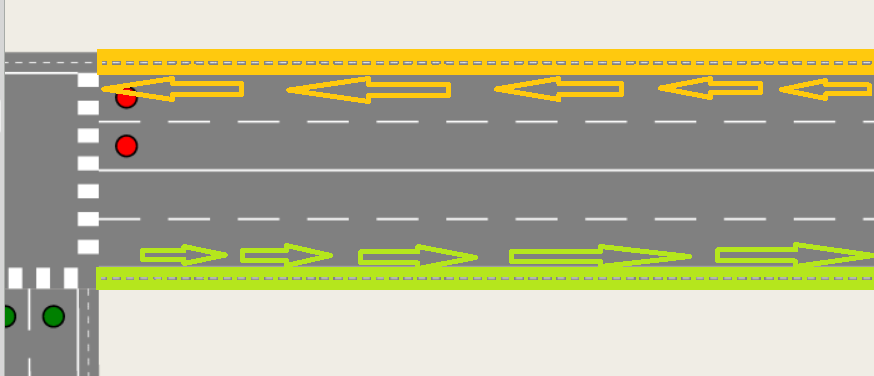
\includegraphics[width=0.9\linewidth]{VersoMarciapiedi}}
\caption{Verso di percorrenza per bici/pedoni.}
\label{fig:Verso di percorrenza per bici/pedoni}
\end{figure}



Le restanti operazioni del protocollo sono operazioni che vanno ripetute per entrambi i versi di percorrenza;
\item per ammortizzare l'operazione di spostamento delle entità passive non conviene spostare prima tutte le entità di tipo pedone e poi tutte le entità di tipo bici; innanzitutto l'ordine con cui le entità vengono spostate riflette un'ordine che segue il verso di percorrenza delle entità e quindi dall'entità più distante dalla fine del verso di percorrenza a quella più vicina alla fine del marciapiede/pista ciclabile. Seguendo la logica del modello IDM nello spostamento di queste entità non è più sufficiente considerare solo la distanza con l'entità successiva (per entità successiva si intende quell'entità che presenta una distanza di percorrenza, rispetto alla traiettoria considerata, maggiore rispetto alla distanza in cui si trova l'entità su cui occorre calcolare l'avanzamento), ma occorre considerare se vi sono degli spostamenti anche sulle traiettorie degli ingressi, al fine di evitare che una entità di tipo pedone/bici intersechi la traiettoria di altre entità in entrata o in uscita dall'ingresso;
\item si prenda quindi la bici o il pedone più distante dalla fine del verso di percorrenza e si iteri quindi su questa scelta per lo spostamento di tutte le entità interessate, di seguito i passi richiesti durante ogni iterazione;
\item si deve considerare la presenza di ingressi su entrambi i lati della strada principale al fine di calcolare la distanza con l'entità successiva; alla prima iterazione è necessario inizializzare quindi, in relazione al verso di percorrenza scelto, il primo ingresso che si incontra alla destra dell'entità, d'ora in poi \textit{ingres\-so\_nel\-lo\_stes\-so\_ver\-so} e il primo ingresso che si incontra alla sinistra dell'entità stessa, d'ora in poi \textit{ingres\-so\_nel\_ver\-so\_op\-pos\-to};   
\item occorre controllare se la destinazione dell'entità, ottenuta al punto \textit{c)}, è un luogo della strada principale stessa o se il luogo di destinazione è un luogo che richiede l'attraversamento di un altro incrocio; questa operazione deve essere effettuata al fine di calcolare la distanza dalla fine della traiettoria del marciapiede/pista ciclabile da percorrere;
\item in relazione agli ingressi \textit{ingres\-so\_nel\-lo\_stes\-so\_ver\-so} e \textit{ingres\-so\_nel\_ver\-so\_op\-pos\-to} l'entità può trovarsi rispetto all'uno o all'altro ingresso in una posizione antecedente o in una posizione successiva; considerando entrambe le tipologie d'ingresso se l'entità, ottenuta al punto \textit{c)}, si trova in una posizione antecedente allora per controllare la posizione della prossima entità occorre controllare gli spostamenti sulle traiettorie a partire dall'ingresso \textit{ingres\-so\_nel\_ver\-so\_op\-pos\-to} e dall'ingresso \textit{ingres\-so\_nel\-lo\_stes\-so\_ver\-so}, altrimenti l'entità si troverà in una posizione successiva rispetto agli ingressi considerati precedentemente (\textit{ingres\-so\_nel\_ver\-so\_op\-pos\-to}, \textit{ingres\-so\_nel\-lo\_stes\-so\_ver\-so}); in questo secondo caso si verificano le condizioni necessarie per abilitare/disabilitare lo spostamento delle entità nella traiettoria usci\-ta\_ri\-tor\-no\_bi\-ci e usci\-ta\_ri\-tor\-no\_pe\-do\-ni, se si considera la tipologia d'ingresso \textit{ingres\-so\_nel\_ver\-so\_op\-pos\-to}, infatti conoscendo le posizioni delle entità successive all'ingresso e le posizioni delle entità precedenti l'ingresso è possibile eseguire lo spostamento delle traiettorie sopra dette, dato che sfruttando le entità precedenti è possibile determinare se la distanza delle entità è tale da permettere l'attraversamento, mentre considerando le entità a distanza maggiore dell'ingresso, ovvero le entità su cui ancora occorre eseguire l'aggiornamento di posizione è possibile determinare la distanza dalla prossima entità per le entità in uscita dalle traiettorie sopra dette; questa operazione e quindi l'aggiornamento dell'ingresso \textit{ingres\-so\_nel\_ver\-so\_op\-pos\-to}, va iterata fintanto che l'entità ottenuta al punto \textit{c)} presenta distanza maggiore dell'ingresso su cui si sta iterando (\textit{ingres\-so\_nel\_ver\-so\_op\-pos\-to}). Le stesse considerazioni possono essere effettuate per gli ingressi del tipo \textit{ingres\-so\_nel\-lo\_stes\-so\_ver\-so}; quindi occorre inserire delle flag per indicare se è possibile o meno permettere la continuazione dell'attraversamento per le entità (bici/pedoni) in entrata nell'ingresso, quindi per quelle bici/pedoni nelle traiettorie \textit{en\-tra\-ta\_drit\-to\_bi\-ci e en\-tra\-ta\_drit\-to\_pe\-do\-ni}, in relazione alle posizioni delle entità che il protocollo è in procinto di spostare, ovvero le entità su cui si sta iterando al punto \textit{c)}; inoltre è necessario disabilitare lo spostamento dei veicoli nelle loro traiettorie per l'ingresso in uscita e in entrata nel caso in cui l'entità pedone/bici intersechi l'attraversamento dei veicoli nelle traiettorie dei veicoli dell'ingresso stesso, dato che i veicoli dovranno dare la precedenza alle bici e ai pedoni che hanno impegnato l'attraversamento dell'ingresso (in questa circostanza dato che la distanza dell'ingresso precede quella dell'entità non occorre considerare la disabilitazione dell'attraversamento dei veicoli nelle traiettorie degli ingressi al fine di permettere il rispetto delle precedenze, dato che entità precedenti sono state già considerate e se necessario avevano già provveduto alle eventuali disabilitazioni per ragioni di precedenza); quindi occorre iterare ed aggiornare \textit{ingres\-so\_nel\-lo\_stes\-so\_ver\-so} fintanto che l'entità considerata in \textit{c)} copra una posizione maggiore dell'ingresso in \textit{ingres\-so\_nel\-lo\_stes\-so\_ver\-so};
\item a questo punto il protocollo ha dato o meno il via libera per lo spostamento di alcune entità; allo stesso tempo è stata eseguita la configurazione di \textit{ingres\-so\_nel\_ver\-so\_op\-pos\-to} e \textit{ingres\-so\_nel\-lo\_stes\-so\_ver\-so} in modo che l'entità ottenuta nello step \textit{c)} abbia una distanza minore agli ingressi appena configurati se ve ne sono;
\item è necessario procedere con il calcolo effettivo della distanza dalla entità successiva:\\
per \textit{ingres\-so\_nel\-lo\_stes\-so\_ver\-so} le traiettorie che l'entità pedone o bici può intersecare sono:
\begin{itemize}
\item tutte le traiettorie in entrata o in uscita dagli ingressi da parte dei veicoli: in particolare ogni veicolo che attraversa una di queste traiettorie, se le sta attraversando significa che nel momento in cui è stata presa la decisione di impegnare la traiettoria non si avevano obblighi di dare precedenza; quindi un pedone/bici percorre la sua pista con la consapevolezza che gli verrà data la precedenza, ma potrebbe succedere che un veicolo abbia impegnato le traiettorie dato che non aveva obblighi di precedenza; così sarà necessario considerare se il veicolo è in una posizione di intersezione nella percorrenza della pista da parte di pedoni/bici; 
\item en\-tra\-ta\_des\-tra\_pe\-do\-ni e en\-tra\-ta\_des\-tra\_bi\-ci; in questo caso occorre considerare anche la lunghezza del veicolo che ha impegnato queste traiettorie;
\item usci\-ta\_des\-tra\_bi\-ci, usci\-ta\_des\-tra\_pe\-do\-ni, usci\-ta\_drit\-to\_bi\-ci e usci\-ta\_drit\-to\_pe\-do\-ni; in questo caso un'entità si troverà davanti all'entità stabilita nel punto \textit{c)} nel momento in cui una enitità pedone o bici stia impegnando una delle traiettorie sopra riportate in un punto che intersechi la percorrenza dei pedoni/bici nella loro pista.
\end{itemize}
per \textit{ingres\-so\_nel\_ver\-so\_op\-pos\-to} le traiettorie che l'entità pedone o bici può intersecare sono:
\begin{itemize}
\item usci\-ta\_ri\-tor\-no\_bi\-ci e usci\-ta\_ri\-tor\-no\_pe\-do\-ni;
\item en\-tra\-ta\_ritorno\_bici e en\-tra\-ta\_ri\-tor\-no\_pe\-do\-ni in questo caso non basta considerare l'intersezione di queste traiettorie con la pista di percorrenza di bici e pedoni, ma occorre considerare la lunghezza delle entità che hanno impegnato le traiettorie sopra esposte.
\end{itemize}
occorre considerare anche la distanza dell'entità considerata al punto \textit{c)} con l'entità successiva che si presenta nella pista, tale entità potrebbe essere o meno presente; se è presente, interrogando la mailbox del task stesso è possibile ricavare la posizione dell'entità successiva; altrimenti occorrerà interrogare la mailbox dell'incrocio successivo al verso di percorrenza dell'entità e quindi ottenere le informazioni relative alla posizione dell'entità che si trova ad impegnare per prima l'incrocio a seconda del tipo di entità richiedente l'informazione.\\
Prendendo poi il minimo tra le precedenti distanze calcolate si ottiene il valore per il parametro della distanza dalla prossima entità da dare in input al modello IDM.
\item eseguito il calcolo e l'aggiornamento della posizione relativa alla fine del quanto di tempo in questione, dovrà essere effettuato l'inserimento dell'entità nella mailbox dell'incrocio stesso interessato se l'entità ha percorso interamente la pista, per convenzione l'inserimento da parte di altre entità fa si che la nuova entità passiva debba essere inserita su una struttura temporanea della mailbox dell'entità interessata all'inserimento;
\item a seconda della posizione dell'entità occorre procedere con l'abilitazione/disabilitazione di eventuali entità (bici/pedoni) che all'incrocio successivo al verso di percorrenza dell'entità definita in \textit{c)} devono effettuare una svolta a sinistra, al fine di permettere il posizionamento nel marciapiede/pista ciclabile appunto di queste entità dell'incrocio che devono svoltare a sinistra (questa parte del protocollo verrà approfondita nel protocollo \ref{spostamentoIncroci});
\item il protocollo durante le iterazioni configura l'ingresso in \textit{ingres\-so\_nel\-lo\_stes\-so\_ver\-so} in modo tale che l'entità passiva, definita in \textit{c)}, si trovi in una posizione antecedente l'ingresso \textit{ingres\-so\_nel\-lo\_stes\-so\_ver\-so}; se l'entità passiva si trova in una posizione che compromette la sicurezza per l'attraversamento di entità di tipo veicolo nelle loro traiettorie in entrata e in uscita dall'ingresso, è necessario disabilitare l'attraversamento di veicoli delle traiettorie negli ingressi per ragioni di precedenza;
\item nel caso siano finite le entità al punto \textit{c)} è necessario considerare se vi sono ancora degli ingressi a partire dallo stato lasciato dalle iterazioni precedenti in \textit{ingres\-so\_nel\-lo\_stes\-so\_ver\-so} e \textit{ingres\-so\_nel\-lo\_stes\-so\_ver\-so}; occorrerà quindi procedere con le abilitazioni/disabilitazioni, viste in precedenza nel protocollo, per lo spostamento delle entità di tipo veicolo, bici o pedone.
\end{enumerate}
\item l'entità attiva dopo aver spostato le entità di tipo bici e pedone in spostamento su marciapiede e piste ciclabili può procedere con lo spostamento dei veicoli presenti sulla strada principale:
\begin{enumerate}
\item una strada principale è composta da 2 corsie per senso di marcia; un'entità deve poter cambiare corsia se necessario, quindi un'entità di tipo veicolo per calcolare la distanza dall'entità che lo precede dovrà considerare anche la possibilità che alcuni veicoli possono cambiare corsia; per queste ragioni l'ordine di spostamento delle entità di tipo veicolo dovrà essere eseguito seguendo l'ordine contrario rispetto al verso di percorrenza delle entità; ovvero partendo dal veicolo più vicino alla fine della strada principale fino al veicolo situato nella parte opposta, ovvero al veicolo più vicino all'inizio del verso di percorrenza considerato (in altre parole dal veicolo che copre la distanza di percorrenza della strada maggiore al veicolo che copre la distanza di percorrenza della strada stessa minore); questa scelta è dovuta al fatto che nel momento in cui un veicolo necessita di cambiare corsia potrà impostare una certa flag per segnalare l'evento; così facendo i veicoli antecedenti al veicolo che ha impostato la flag (con antecedenti si intende quei veicoli che coprono una posizione minore nella strada principale rispetto al veicolo considerato), nel calcolare la distanza con l'entità successiva potranno considerare immediatamente, senza attendere il quanto di tempo successivo, quei veicoli che sono in cambio corsia, evitando così situazioni di avanzamento inaspettate;
\item i veicoli devono essere quindi spostati seguendo l'ordine indicato al punto precedente; dato che esistono 2 corsie comunque si deve iterare sull'entità più distante tra le 2 corsie al netto dei veicoli su cui è già stata eseguita l'iterazione;
\item un veicolo deve seguire una certa destinazione e il luogo di destinazione potrebbe trovarsi nella strada principale in esame, oppure la destinazione potrebbe essere in un'altra strada principale e quindi il veicolo dovrà percorrere tutta la strada principale;
\item il veicolo si troverà in una certa corsia, quella su cui è stato inserito da parte dell'entità ingresso o dell'entità incrocio (il primo caso si presenta se il veicolo ha come luogo di partenza un luogo appartenente alla strada principale in esame). La corsia nel quale è stato inserito il veicolo non è per forza la corsia corretta in cui il veicolo deve essere gestito al fine di raggiungere la destinazione stabilita per il veicolo; il veicolo dovrà contenere dei parametri che dovranno indicare la corsia di provenienza del veicolo stesso e la corsia di destinazione, questi parametri dovranno essere correttamente configurati nel momento in cui l'entità veicolo viene inserita nella mailbox dell'entità strada principale;
\item l'entità, preso il veicolo ottenuto dall'iterazione al punto \textit{b)} del protocollo, deve controllare la corsia di destinazione del veicolo. Se la corsia di destinazione del veicolo è diversa dalla corsia in cui il veicolo stesso si trova occorre dapprima calcolare la distanza limite in cui può avvenire il cambio corsia; la distanza limite viene fissata al fine di permettere una gestione controllata dei cambi corsia; il valore che limita la distanza viene impostato in modo consono con il modello della mappa; per esempio nel caso in cui un veicolo deve muoversi tra 2 luoghi che appartengono alla stessa strada principale, se deve essere eseguito il cambio corsia si deve presentare la situazione in cui la distanza tra i 2 luoghi sia tale da permettere il completamento della traiettoria di cambio corsia e inoltre sia tale da essere maggiore della distanza limite scelta dal sistema per l'esecuzione del cambio corsia. Tale distanza limite è una distanza da considerare dal luogo di destinazione, quindi entro quella distanza dal luogo di destinazione deve essere eseguito il cambio corsia. Nel caso in cui non è stato possibile effettuare il cambio corsia entro la distanza limite, il veicolo dovrà attendere, nel punto indicato come di distanza limite, il verificarsi delle condizioni per poter eseguire il cambio corsia; se il veicolo (V\_A) deve effettuare il cambio corsia ma la sua posizione non ha ancora raggiunto la distanza limite, allora il task valuterà se V\_A potrà effettuare il cambio corsia. Per l'esecuzione del cambio corsia da parte di V\_A viene valutata se la posizione del veicolo V\_B posto nella corsia di destinazione per il cambio corsia di V\_A ad una distanza minore di V\_A stesso sia ad una distanza tale da permettere una manovra di cambio corsia senza incidenti; se nella corsia di destinazione di V\_A non esiste alcun veicolo V\_C situato a distanza maggiore di V\_A allora si può continuare a valutare le altre condizioni per abilitare il cambio corsia, altrimenti si deve valutare la velocità di V\_C rispetto alla velocità del veicolo V\_D situato ad una posizione successiva nella corsia in cui si trova V\_A, e quindi le loro distanze da V\_A al fine di permettere al veicolo V\_A di trarre il massimo vantaggio nell'avanzamento dopo il cambio corsia. Se fin qui le condizioni per eseguire il cambio corsia sono favorevoli si deve procedere con la valutazione della presenza di eventuali veicoli in intersezione con la traiettoria di cambio corsia, quindi se l'insieme delle intersezioni è vuoto si dovrà calcolare se il veicolo si trova in prossimità di un ingresso; infatti nel caso in cui il veicolo si trovi in prossimità di un ingresso in cui sono in luogo degli spostamenti di una qualche entità, allora il cambio corsia non può avvenire a meno che il completamento della traiettoria di cambio corsia sia precedente alla distanza in cui l'ingresso in prossimità di V\_A sia situato; nel caso queste condizioni non siano valide il cambio corsia deve essere ritardato e al più avverrà per raggiungimento della distanza limite della destinazione di V\_A;\\
la scelta del porre un limite entro il quale eseguire il cambio corsia potrebbe portare ad una situazione di stallo in cui esistano 2 veicoli situati su corsie diverse che hanno raggiunto entrambi il limite per eseguire il cambio corsia; si noti che l'unico caso per cui questa situazione può succedere, per come è costruita la mappa è se la destinazione dei veicoli interessati non si trova nella strada principale in esame; infatti dato che gli ingressi sulla strada principale sono situati ad una distanza minima l'uno dall'altro fissata a priori, per potersi verificare una situazione di stallo sarebbe necessario che un veicolo situato nella corsia più a destra debba cambiare corsia per poter raggiungere l'ingresso nel lato opposto della strada, e un veicolo situato nella corsia più a sinistra, sempre relativa al verso di percorrenza, debbe cambiare corsia per raggiungere l'ingresso posto nel lato della strada principale che si trova alla destra del verso di percorrenza del veicolo, inoltre deve succedere che entrambi i veicoli abbiano raggiunto il limite per cambio corsia; in questo caso si avrebbe una situazione di stallo, tuttavia dato che la mappa non prevede una configurazione in cui 2 ingressi siano l'uno di fronte all'altro la situazione non potrà verificarsi. \\
Questa situazione invece potrebbe verificarsi se il limite per eseguire il cambio corsia si presenta nel caso in cui 2 veicoli presenti su corsie diverse abbiano raggiunto la distanza limite dall'incrocio (considerando che entrambi i veicoli devono attraversare l'incrocio). La situazione sarebbe la seguente: un veicolo che si trova nella corsia più a destra rispetto al suo verso di percorrenza deve prendere al prossimo incrocio la traiettoria di sinistra e quindi dovrà effettuare il cambio corsia, dall'altra parte si ha un veicolo situato nella corsia più a sinistra rispetto al suo verso di percorrenza che al prossimo incrocio dovrà svoltare a destra. Se entrambi i veicoli hanno raggiunto il limite per sorpassare è necessario stabilire la regola della precedenza a destra; ovvero il veicolo situato nella corsia più a sinistra (V\_A) dovrà aspettare il passaggio del veicolo situato più a destra, e quest'ultimo dovrà eseguire il cambio corsia anche se le condizioni di distanza minima dal veicolo V\_A non sono rispettate;
\item se il veicolo si trova in stato di sorpasso occorre procedere con l'avanzamento del sorpasso stesso; altrimenti il veicolo si troverà nella corsia corretta rispetto alla destinazione da raggiungere e quindi si può procedere con l'avanzamento esposto nei punti successivi;  
\item al modello finora esposto per la gestione del cambio corsia può essere adattato un modello che permetta effettivamente dei sorpassi tra i veicoli; il modello finora visto si basa sulla considerazione che un veicolo è configurato con una certa corsia di partenza e una certa corsia di destinazione ed il protocollo ha come obiettivo quello di portare il veicolo alla corsia desiderata; giocando su questo fatto è possibile introdurre i sorpassi cambiando il valore della corsia di destinazione a seconda del verificarsi di alcune condizioni che sono favorevoli all'esecuzione dei sorpassi, il valore corretto poi della corsia di destinazione dovrà essere correttamente ripristinato al fine di permettere al veicolo di raggiungere la corretta destinazione. Ai punti precedenti del protocollo quindi dovranno essere aggiunti i controlli per gestire e cambiare la corsia di destinazione dei veicoli per permettere l'esecuzione dei sorpassi;
\item il task deve occuparsi anche del calcolo della distanza dall'entità successiva che un veicolo incontra; se l'abitante si trova in stato di sorpasso allora la distanza dall'entità successiva va calcolata rispetto alla corsia di destinazione del sorpasso, inoltre dato che un sorpasso non può essere effettuato nel caso esista qualche entità intersecante la traiettoria di sorpasso, si avrà che la distanza dalla prossima entità sarà in una posizione successiva alla lunghezza della traiettoria di sorpasso;
per valutare quindi la distanza che un veicolo ha dall'entità successiva si deve prendere il valore minimo delle distanze calcolate tra le seguenti entità:
\begin{itemize}
\item la distanza rispetto al veicolo che si trova nella corsia di destinazione del veicolo per il quale è in corso il calcolo della posizione della prossima entità; per calcolare tale distanza non ci si può limitare a calcolare la distanza dalla prossima macchina in corsia, ma si deve considerare anche se veicoli appartenenti alla corsia opposta sono in stato di sorpasso (da ricordare che l'entità su cui è in corso l'aggiornamento di posizione, per come vengono eseguiti gli aggiornamenti di posizione, ha la conoscenza dell'avvenimento del sorpasso di un'entità direttamente nel quanto di sistema in corso);
\item la distanza rispetto a eventuali entità in movimento su una qualche traiettoria in entrata o in uscita da un ingresso situato in uno qualunque dei 2 lati della strada principale. 
\end{itemize}
\item nel caso in cui un veicolo debba percorrere tutta la traiettoria della strada principale, il sistema dell'avanzamento permette al veicolo di raggiungere in un certo quanto una posizione ravvicinata alla fine della strada principale; l'obiettivo è quello di permettere un avanzamento fluido dall'entità della strada principale, all'entità incrocio. Quindi una volta raggiunta tale posizione il task dovrà interagire con la mailbox dell'incrocio di destinazione del veicolo (V\_A) al fine di apprendere la distanza dalla prima entità presente nella traiettoria che V\_A dovrà intraprendere; questa operazione può essere iniziata se il semaforo dell'incrocio è verde per il veicolo V\_A. Il valore ritornato dalla richiesta alla mailbox dell'incrocio non potrà essere subito validato: infatti potrebbe succedere la seguente situazione: l'incrocio non ha nessun veicolo in movimento; oltre a V\_A esiste un veicolo V\_B situato nella strada opposta a quella di V\_A, supponendo che V\_A si trovi nella corsia più a sinistra e deve procedere in direzione dritto nell'incrocio, mentre V\_B si trova anch'esso nella corsia più a sinistra e deve procedere nella traiettoria sinistra, in modo tale che le traiettorie di V\_A e V\_B possano intersecarsi. Il problema quindi è che il task gestore di V\_A non conosce ciò che il task di V\_B sta facendo e viceversa, quindi potrebbe verificarsi un incidente tra i 2 veicoli; è necessario limitare la distanza ottenuta in risposta dalla mailbox dell'incrocio in funzione delle distanze di intersezione con le traiettorie dell'incrocio che le entità devono percorrere;
\item se il veicolo ha percorso interamente la strada principale, il task dovrà comunicare al gestore del servizio di locazione del veicolo che il task ha percorso interamente la strada principale, infine il veicolo dovrà essere inserito nella mailbox dell'entità incrocio in modo tale che al prossimo quanto di sistema l'entità incrocio potrà gestire il nuovo veicolo;
\item ogni entità (V\_A)che deve essere spostata contribuisce alla determinazione per l'abilitazione degli spostamenti per le entità in uscita o in entrata dagli ingressi; in particolare il sistema prevede l'abilitazione/disabilitazione per le entità di tipo bici/pedone che sono in procinto di iniziare l'attraversamento verso il primo pezzo dell'attraversamento pedonale, o che sono situate a metà dell'attraversamento pedonale e che intendono continuare l'attraversamento. Quindi un'entità rispetto ad un certo ingresso potrà trovarsi in una posizione successiva o antecedente; nel primo caso se l'entità interseca parte dell'attraversamento pedonale dell'ingresso sarà necessario disabilitare l'attraversamento di entità (pedoni/bici) in uscita dall'ingresso (per traiettorie \textit{usci\-ta\_drit\-to\_bi\-ci e usci\-ta\_drit\-to\_pe\-do\-ni} di ingressi situati alla destra di V\_A) o in entrata nell'ingresso (per traiettorie \textit{en\-tra\-ta\_ri\-tor\-no\_bi\-ci e en\-tra\-ta\_ri\-tor\-no\_pe\-do\-ni} per ingressi situati alla sinistra di V\_A). Altrimenti V\_A si troverà ad una distanza minore a quella della fine dell'ingresso: in questo caso ci sono diversi elementi che contribuiscono all'abilitazione all'attraversamento:
\begin{itemize}
\item per l'abilitazione delle traiettorie di bici/pedoni in entrata/uscita dagli ingressi presenti al lato destra dell'entità V\_A, lo spostamento deve essere abilitato se non vi sono dei veicoli la cui posizione al quanto corrente o al quanto successivo non violi la distanza di sicurezza per permettere l'attraversamento, la regola vale considerando sia veicoli appartenenti indifferentemente all'una o all'altra corsia, sia per veicoli in sorpasso; tale regola è soggetta ad un'eccezione, infatti nel caso in cui ci siano delle entità (pedoni/bici) che sono in attraversamento nelle traiettorie di en\-tra\-ta\_drit\-to\_bi\-ci e en\-tra\-ta\_drit\-to\_pe\-do\-ni, si avrà che i veicoli stanno dando la precedenza a tali entità, quindi la disabilitazione degli attraversamenti per le entità in usci\-ta\_drit\-to\_bi\-ci e usci\-ta\_drit\-to\_pe\-do\-ni non deve avvenire; infine è necessario procedere con l'abilitazione/disabilitazione per le entità che si trovano nel secondo pezzo delle traiettorie en\-tra\-ta\_drit\-to\_bi\-ci e en\-tra\-ta\_drit\-to\_pe\-do\-ni in cui la regola per l'abilitazione segue qui solo il controllo che le entità di tipo V\_A sia a distanza sufficiente da permettere l'attraversamento di bici e pedoni nelle traiettorie di entrata nell'ingresso;
\item per l'abilitazione delle traiettorie per gli ingressi presenti al lato sinistro dell'entità V\_A  la procedura è simmetrica al caso precedente solamente che le traiettorie che richiedono l'abilitazione saranno il primo pezzo dell'attraversamento per en\-tra\-ta\_drit\-to\_bi\-ci e en\-tra\-ta\_drit\-to\_pe\-do\-ni e il secondo pezzo dell'attraversamento per le traiettorie usci\-ta\_drit\-to\_bi\-ci e usci\-ta\_drit\-to\_pe\-do\-ni;
\item altre entità che potrebbero provocare l'avvenimento inaspettato di incidenti è evitato dai seguenti controlli: per entità (bici/pedoni) che sono gestite nelle traiettorie usci\-ta\_drit\-to\_bi\-ci e usci\-ta\_drit\-to\_pe\-do\-ni, in avanzamento nel primo pezzo dell'attraversamento dovrà avvenire la disabilitazione nel caso in cui esistano veicoli che hanno già iniziato a muoversi nella traiettoria usci\-ta\_an\-da\-ta affinchè tali veicoli intersechino l'attraversamento; analogamente per le bici/pedoni in avanzamento nel secondo pezzo dell'attraversamento pedonale dovrà avvenire la disabilitazione nel caso in cui esistano veicoli che hanno già iniziato a muoversi nella traiettoria en\-tra\-ta\_ri\-tor\-no affinchè tali veicoli intersechino l'attraversamento; il caso simmetrico viene a presentarsi per le intersezioni tra la traiettoria usci\-ta\_ri\-tor\-no dei veicoli e l'attraversamento nel primo pezzo dell'attraversamento pedonale da parte di entità (bici/pedoni) nelle traiettorie en\-tra\-ta\_ri\-tor\-no\_bi\-ci e en\-tra\-ta\_ri\-tor\-no\_pe\-do\-ni, e infine l'intersezione tra la traiettoria dei veicoli situati nella traiettoria en\-tra\-ta\_an\-da\-ta con le entità (bici/pedoni) in percorrenza nel secondo pezzo dell'attraversamento delle traiettorie en\-tra\-ta\_drit\-to\_bi\-ci e en\-tra\-ta\_drit\-to\_pe\-do\-ni.
\end{itemize}
\item quando l'insieme delle entità definito in \textit{b)} è vuoto si può procedere con la disabilitazione effettiva delle entità (bici/pedoni) in entrata o in uscita dagli ingressi, così da permettere se possibile gli avanzamenti delle entità direttamente nel quanto di sistema corrente.
\end{enumerate}
\item a questo punto i punti precedenti del protocollo hanno abilitato se possibile gli spostamenti per le entità in gestione alle traiettorie degli ingressi;
\item l'entità attiva si occupa poi della gestione degli spostamenti per le entità presenti nelle traiettorie degli ingressi adibite allo spostamento di bici e pedoni:
\begin{enumerate}
\item ogni ingresso possiede delle traiettorie; un ingresso può essere situato su uno dei 2 lati della strada principale gestita dall'entità attiva in questione; lo spostamento per le entità in queste traiettorie può seguire un qualunque ordine rispetto alla disposizione degli ingressi appartenenti a un lato o all'altro; l'ordine scelto è quello di spostare le entità delle traiettorie degli ingressi, prima rispetto a tutti quelli di un certo lato, poi passando alla gestione degli spostamenti per ingressi situati al lato opposto; in questo modo è possibile considerare una sola volta le entità presenti nel marciapiede/pista ciclabile al fine di determinare le precedenze nell'avanzamento delle entità sulle traiettorie in uscita o in entrata dell'ingresso stesso;
\item iterando quindi sugli ingressi prima di un lato, poi dell'altro della strada principale si dovrà eseguire lo spostamento delle entità presenti nelle seguenti traiettorie:
\begin{itemize}
\item \textit{en\-tra\-ta\_ri\-tor\-no\_bi\-ci e en\-tra\-ta\_ri\-tor\-no\_pe\-do\-ni}: un'entità presente in questa tipologia di traiettoria potrà avanzare solo se nella medesima traiettoria non vi sono altre entità già impegnate nell'avanzamento nella medesima traiettoria; inoltre l'avanzamento per queste entità deve essere abilitato, dipendentemente dallo stato di avanzamento delle entità nella strada principale, così da permettere il controllo del fatto che l'entità bici/pedone non incorra in incidenti inaspettati. L'abilitazione quindi deve avvenire nel momento in cui viene gestito lo spostamento dei veicoli nella strada principale; se l'entità è abilitata allo spostamento, per certo otterrà la precedenza dai veicoli presenti sulla strada principale, quindi quando la traiettoria è stata interamente percorsa dopo l'aggiornamento delle posizioni delle entità che avverrà dopo la nuova sincronizzazione verrà spostata l'entità dalle traiettorie qui esaminate alle traiettorie \textit{en\-tra\-ta\_drit\-to\_pe\-do\-ni e en\-tra\-ta\_drit\-to\_bi\-ci}, così da permettere che al nuovo quanto di tempo la gestione delle entità interessate avvenga dalle traiettorie appena riportate;
\item \textit{en\-tra\-ta\_drit\-to\_pe\-do\-ni e en\-tra\-ta\_drit\-to\_bi\-ci}: un attraversamento pedonale coinvolge entrambi i sensi di marcia della strada principale, quindi l'attraversamento sarà caratterizzato da 2 parti suddivise dalla linea che delimita il senso di marcia; il sistema di precedenze sugli attraversamenti pedonali si basa sul fatto che delle entità di tipo veicolo nel momento in cui ci siano dei pedoni o bici nelle traiettorie in \textit{en\-tra\-ta\_ri\-tor\-no\_bi\-ci e en\-tra\-ta\_ri\-tor\-no\_pe\-do\-ni} con flag di abilitazione, allora i veicoli presenti su una qualunque delle corsie (della strada principale) interesecanti la prima parte dell'attraversamento pedonale daranno la precedenza; la precedenza da parte dei veicoli nella corsia più a sinistra verrà data fintanto che esistano delle bici o dei pedoni nelle traiettorie in descrizione purchè intersechino una parte della corsia interessata, analogamente per i veicoli nella corsia più a destra del senso di marcia considerato; il ragionamento è analogo per i veicoli nel senso di marcia opposto, solamente che questi daranno la precedenza solamente nel caso in cui le entità di tipo bici e pedoni in attraversamento sulla zona della corsia più a destra della prima parte dell'attraversamento pedonale, abbiano l'abilitazione della flag di spostamento anche sulla seconda parte dell'attraversamento pedonale, che dovrà essere data se possibile nel momento in cui vengono spostate le entità che percorrono la strada principale in intersezione con la seconda parte dell'attraversamento pedonale. È possibile applicare un'ottimizzazione in realtà per quelle entità (bici/pedone) che necessitano dell'abilitazione per attraversare la seconda parte dell'attraversamento pedonale; ovvero nel momento in cui un'entità (bici/pedone) intersechi la corsia più a sinistra della seconda parte dell'attraversamento pedonale allora sicuramente i veicoli che vogliono attraversare la seconda parte dell'attraversamento pedonale stanno dando la precedenza a quell'entità, e quindi un entità (bici/pedone) situata nella corsia più a sinistra della prima parte dell'attraversamento pedonale potrà ottenere l'abilitazione all'attraversamento. Un'entità situata in una di queste traiettorie dovrà percorrere la traiettoria fino al raggiungimento del marciapiede/pista ciclabile da cui poi dovrà attendere l'abilitazione per completare l'attraversamento, che sarà data dal protocollo descritto al punto \textit{2.f}; infine a traiettoria completata occorre eseguire l'inserimento dell'entità nella mailbox dell'ingresso che l'entità interessata deve raggiungere. Per ottenere effettivamente l'abilitazione per eseguire l'attraversamento occorre integrare al punto \textit{2.f} il fatto che non vi siano entità nelle traiettorie in en\-tra\-ta\_des\-tra\_bi\-ci ed en\-tra\-ta\_des\-tra\_pe\-do\-ni; l'effettiva abilitazione agli spostamenti avviene quindi alla fine del protocollo descritto in \textit{2};
\item \textit{en\-tra\-ta\_des\-tra\_bi\-ci e en\-tra\-ta\_des\-tra\_pe\-do\-ni}: le condizioni per permettere lo spostamento di entità appartenenti a queste traiettorie sono: l'assenza di altre entità in movimento nella medesima traiettoria, l'assenza di entità nei marciapiedi/pista ciclabile in intersezione con le traiettorie in descrizione, l'assenza di entità con flag abilitato a True per permettere il completamento dell'attraversamento delle traiettorie in \textit{en\-tra\-ta\_drit\-to\_pe\-do\-ni e en\-tra\-ta\_drit\-to\_bi\-ci}; validate le condizioni dovrà essere calcolata la posizione dell'entità successiva che se presente sarà la prima entità, della tipologia interessata, in entrata nel marciapiede/pista ciclabile nel verso che segue l'uscita dalla strada principale;
\item \textit{usci\-ta\_des\-tra\_bi\-ci e usci\-ta\_des\-tra\_pe\-do\-ni}: per le entità inserite dall'ingresso in queste traiettorie dovrà essere calcolata la presenza o meno di altre entità in percorrenza nel marciapiede/pista ciclabile in intersezione con le medesime traiettorie considerate o altrimenti se tali entità presentano una distanza sufficiente dalle traiettorie in descrizione al fine di permetterne l'attraversamento di evenutali entità presenti; occorre poi accertarsi del fatto che non esistano delle entità appartenenti a \textit{usci\-ta\_drit\-to\_bi\-ci e usci\-ta\_drit\-to\_pe\-do\-ni} che risultino in intersezione con le traiettorie in descrizione; se tali condizioni sono valide occorrerà considerare se esistono altre entità in percorrenza le traiettorie in descrizione, quindi se non ne esistono allora lo spostamento può avvenire. Per calcolare la posizione dell'entità successiva occorre considerare non più solo la presenza dell'entità dello stesso tipo che si trova a distanza maggiore dell'ingresso e quindi in gestione sulla stessa tipologia di risorsa (marciapiede/pista ciclabile), ma si dovrebbe considerare la presenza di eventuali entità presenti su ingressi (considerando ingressi di entrambi i lati); questo fatto porterebbe ad una dipendenza che romperebbe la logica dell'ordinamento che il protocollo in analisi sta imponendo; pertanto è necessario fissare una distanza massima data dalla distanza dal successivo ingresso, se presente, che l'entità dovrà attraversare, considerando gli ingressi posti in entrambi i lati della strada principale. Quindi il parametro della distanza dalla prossima entità da dare in input al modello IDM sarà calcolato come il minimo tra la distanza dal prossimo ingresso che l'entità incontra, indipendentemente dal fatto che esistano o meno delle entità in movimento su questo, e la distanza della prossima entità che viene a trovarsi nel marciapiede/pista ciclabile in una posizione successiva all'entità da spostare; 
\item \textit{usci\-ta\_drit\-to\_bi\-ci e usci\-ta\_drit\-to\_pe\-do\-ni}: le entità appartenenti a queste traiettorie dovranno impegnare l'attraversamento pedonale, quindi dapprima devono ottenere l'abilitazione per l'attraversamento, analogamente a come veniva fatto per \textit{en\-tra\-ta\_ri\-tor\-no\_pe\-do\-ni e en\-tra\-ta\_ri\-tor\-no\_bi\-ci}; quindi nel momento in cui viene gestito l'avanzamento per le entità che si trovano nella strada principale dovranno essere valutate alcune condizioni per permettere l'abilitazione all'attraversamento per le entità presenti nelle traiettorie in descrizione (tali condizioni verranno esaminate nei punti successivi degli step dell'entità attiva in esame). L'attraversamento pedonale coperto dalle traiettorie in descrizione si divide in 2 parti, dove ogni parte è separata dalla linea che divide il senso di percorrenza dei veicoli nella strada principale. Quindi un veicolo che si trova in movimento nella strada principale e che interseca il primo pezzo dell'attraversamento pedonale darà la precedenza alle entità che hanno ottenuto l'abilitazione allo spostamento fintanto che le entità nelle traiettorie in descrizione precedono la corsia sulla quale il veicolo è inserito e fintanto che tali entità intersecano parte della corsia interessata; quindi un'entità per poter poi continuare l'attraversamento oltre la linea che separa i sensi di marcia della strada principale dovrà ottenere una nuova abilitazione, questa volta l'abilitazione dovrà essere data dall'entità attiva stessa nel momento in cui vengono spostati i veicoli che nel loro percorso intersecano la seconda parte dell'attraversamento pedonale. Anche qui è possibile ottimizzare sull'abilitazione nell'attraversamento; in particolare la prima abilitazione può essere data se esiste un'entità (bici/pedone) che è in intersezione con la corsia più a sinistra che interseca il primo pezzo dell'attraversamento pedonale; mentre la seconda abilitazione può essere data nel momento in cui l'entità (bici/pedone) si trovi nella corsia più a sinistra che interseca il primo pezzo dell'attraversamento pedonale purchè esista un'entità (bici/pedone) in intersezione con la corsia più a sinistra del secondo pezzo dell'attraversameno pedonale dato che per queste entità i veicoli devono già dare la precedenza. La traiettoria dovrà poi quindi essere completamente attraversata da parte delle entità (bici/pedone) ed aspettare l'abilitazione vista nel protocollo \textit{2.f} per impegnare prima le traiettorie \textit{usci\-ta\_ri\-tor\-no\_bi\-ci e usci\-ta\_ri\-tor\-no\_pe\-do\-ni} e poi le risorse marciapiede/pista ciclabile;
\item \textit{usci\-ta\_ri\-tor\-no\_bi\-ci e usci\-ta\_ri\-tor\-no\_pe\-do\-ni}: un'entità che si trova in gestione a queste traiettorie se si trova in posizione 0 deve controllare se le entità (bici/pedoni) che sono in movimento presso il marciapiede/pista ciclabile in cui le entità in gestione alle traiettorie in descrizione devono essere inserite, si trovino ad una distanza tale da abilitare lo spostamento per le entità in posizione 0; la validità della condizione sopra riportata e il controllo dell'assenza di intersezioni delle traiettorie in descrizione con altre entità in movimento sulla risorsa (marciapiede/pista ciclabile) in cui le entità devono essere spostate fa si che sia possibile abilitare lo spostamento per le entità in posizione 0. Quindi occorre calcolare poi la distanza dalla prossima entità che verrà a trovarsi in una posizione successiva della distanza della traiettoria in esame (distanza intesa come riferita alla locazione della traiettoria nella strada principale); la distanza calcolata deve però essere limitata al più dalla distanza del primo ingresso successivo che l'entità, inserita nella risorsa marciapiede/pista ciclabile, incontrerebbe al fine di evitare dipendenze sull'ordine di esecuzione degli spostamenti tra ingressi.
\end{itemize}
\end{enumerate}
\item le entità che restano da spostare sono i veicoli presenti in entrata o in uscita dagli ingressi; tali veicoli hanno, se possibile, già ottenuto per il quanto di sistema corrente l'abilitazione allo spostamento, in modo da evitare incidenti con le entità di tipo bici/pedone in avanzamento su marciapiede/pista ciclabile della strada principale; di seguito i passi da eseguire per permettere l'avanzamento dei veicoli in entrata o in uscita dalle traiettorie degli ingressi (gestite dal task della strada principale):
\begin{itemize}
\item \textit{u\-sci\-ta\_an\-da\-ta}: per un'entità (V\_A) presente in una traiettoria di questo tipo, può essere avviato lo spostamento se la traiettoria stessa non è impegnata da altre entità; poi occorre controllare se i veicoli hanno ricevuto l'abilitazione allo spostamento (nel caso quindi in cui non vi sono delle bici/pedoni in attraversamento sull'ingresso in un punto che non interseca la traiettoria in descrizione); se non ci sono bici/pedoni che sono in attraversamento nella corsia di destinazione di V\_A si può continuare con il prossimo controllo ovvero si deve controllare se esiste un veicolo in spostamento nella traiettoria \textit{usci\-ta\_ri\-tor\-no} in una posizione che intersechi la traiettoria in descrizione. Infine si deve considerare se la posizione aggiornata dei veicoli su strada è ad una distanza tale da non permettere l'attraversamento della traiettoria in sicurezza o se esistano altri veicoli che intersechino la traiettoria in descrizione, per monitorare se l'attraversamento avviene in sicurezza occorre anche considerare l'eventuale presenza di veicoli in sorpasso dalla corsia opposta alla corsia di destinazione di V\_A; infine se tutti i controlli sono andati a buon fine si può procedere con il calcolo della posizione della prossima entità che V\_A incontrerebbe se dovesse essere inserito nella strada principale;
\item \textit{usci\-ta\_ri\-tor\-no}: un'entità (V\_A) che deve essere spostata in una traiettoria di questo tipo, può analogamente a prima essere spostata se non vi sono altre entità presenti nella stessa traiettoria; occorre poi valutare se per veicoli in questa tipologia di traiettoria è stata data l'abilitazione allo spostamento (dai protocolli precedenti) per evitare quindi incidenti con bici/pedoni; la percorrenza della traiettoria in descrizione dovrà essere interrotta nel punto di intersezione della traiettoria con la prima corsia incontrata nel caso in cui esistano delle entità in sorpasso verso la corsia in cui V\_A è in procinto di muoversi o nel caso in cui esistano dei veicoli in percorrenza su quella corsia tali che per entrambi i casi presentano una distanza troppo ravvicinata per permettere a V\_A di continuare l'attraversamento. Quindi in questi casi V\_A dovrà fermarsi e dare la precedenza a quelle entità, altrimenti potrà proseguire controllando prima se occorre dare la precedenza a veicoli presenti nella traiettoria \textit{en\-tra\-ta\_ri\-tor\-no}, quindi se necessario fermarsi poi nel punto di intersezione della traiettoria con la linea divisoria dei sensi di marcia di percorrenza dei veicoli e validare le condizioni per l'attraversamento considerando le distanze dall'ingresso in questione dei veicoli provenienti dal senso di marcia opposto, sia in sorpasso che non, verso la corsia interessata dalla traiettoria del veicolo V\_A. Infine se non vi sono pedoni o bici in attraversamento nel primo pezzo della traiettoria \textit{en\-tra\-ta\_drit\-to\_bi\-ci} e \textit{en\-tra\-ta\_drit\-to\_pe\-do\-ni} il veicolo potrà completare l'attraversamento della traiettoria e quindi procedere con il calcolo della prossima entità che il veicolo incontrerà una volta inserito nella corsia di destinazione della traiettoria in descrizione; un veicolo che finisce l'attraversamento della traiettoria in descrizione e che quindi dovrà essere inserito nella strada principale, grazie ai controlli sopra riportati avrà come entità successiva, un'entità che si troverà a distanza maggiore della fine della traiettoria in descrizione permettendo quindi di avere delle distanze sempre positive;\\
la stessa considerazione va fatta per ogni entità veicolo, bici, pedone in uscita da una qualunque traiettoria;
\item \textit{en\-tra\-ta\_ri\-tor\-no}: un'entità (V\_A) gestita da una traiettoria di questo tipo può essere spostata se non vi sono altre entità in movimento sulla traiettoria stessa; le entità su questa traiettoria dovranno dare la precedenza a quelle entità presenti sulle corsie con senso di marcia opposto a quello di provenienza dell'entità gestita dalla traiettoria in descrizione, quindi dovranno essere considerati sia veicoli in sorpasso che non, verso la prima corsia di destinazione di V\_A; la traiettoria in descrizione troverà poi l'intersezione con la traiettoria \textit{usci\-ta\_ri\-tor\-no} sulla quale avrà la precedenza a meno che non vi siano già delle entità in avanzamento su quest'ultima traiettoria in una posizione che supera l'obbligo di dare precedenza da parte delle loro entità; il task dovrà poi, se necessario, interrompere l'avanzamento di V\_A, nel punto di intersezione con la linea delimitativa la seconda corsia che la traiettoria incontra; dovrà quindi essere eseguito il controllo della presenza di eventuali veicoli in attraversamento nella traiettoria \textit{en\-tra\-ta\_an\-da\-ta} sui quali occorre dare precedenza (se esistono) altrimenti dovrà essere data precedenza ad altri veicoli in percorrenza la corsia di destinazione di V\_A che violino la distanza di sicurezza per l'attraversamento di V\_A, infine occorre fermare l'entità nel caso in cui sia stato disabilitato l'attraversamento (da parte dei punti precedenti del protocollo) a causa dell'attraversamento dell'ingresso da parte di bici/pedoni (da notare che se un pedone/bici ha disabilitato l'attraversamento per la traiettoria in descrizione allora non esisteva alcuna sua entità V\_A in una posizione che aveva superato la distanza entro la quale poteva essere data la precedenza, d'altro canto un'entità in movimento sulla traiettoria in descrizione dovrà ottenere prima l'abilitazione per poter proseguire nell'avanzamento, e quindi le precedenze sono controllate, dato che l'esecuzione dell'avanzamento è soggetto a precondizioni, nel caso avvenga l'avanzamento sarà questo evento a rallentare le entità che prima avevano la precedenza, permettendo cosi l'avanzamento di tutte le entità e la gestione corretta delle precedenze, dovuta all'ordine stabilito nell'esecuzione dei protocolli); l'entità V\_A durante l'avanzamento deve richiedere alla mailbox dell'ingresso la posizione della prima entità che sta percorrendo l'ingresso nel verso del luogo di destinazione da raggiungere, cosi da permettere un'avanzamento fluido nel passaggio di entità passive tra entità attive; a traiettoria completata il veicolo dovrà essere inserito nella mailbox dell'ingresso per il quale occorrerà eseguire l'avanzamento dal quanto di tempo successivo;
\item \textit{en\-tra\-ta\_an\-da\-ta}: un'entità (V\_A) gestita da traiettorie di questo tipo potrà essere spostata se non vi sono altre entità già in gestione dalla traiettoria in descrizione; occorre controllare se i protocolli precedenti hanno dato l'abilitazione per il completamento dell'attraversamento e inoltre è necessario controllare se sono presenti delle entità (pedone/bici) in percorrenza nel secondo pezzo della traiettorie \textit{en\-tra\-ta\_drit\-to\_bi\-ci e en\-tra\-ta\_drit\-to\_pe\-do\-ni}; il task non permetterà quindi l'avanzamento dell'entità se uno dei precedenti controlli è violato, infine si dovrà controllare se esiste un'entità in \textit{en\-tra\-ta\_ri\-tor\-no} che viene a trovarsi in una posizione tale da non permettere di dare la precedenza a entità nella traiettoria in descrizione; quindi potrà essere calcolato per l'entità la posizione della prossima entità che si troverà nella corsia di destinazione dell'ingresso che V\_A deve raggiungere.
%la regola usata per la rimozione delle entità presenti in en\-tra\-ta\_an\-da\-ta e en\-tra\-ta\_ri\-tor\-no che sono passate in gestione alla mailbox dell'ingresso di destinazione prevede che un veicolo su queste traiettorie potrà essere rimosso solamente nel momento in cui il veicolo si troverà interamente, cioè in toto alla sua lunghezza, nell'ingresso di destinazione; il fine di questa
\end{itemize}
\item prima della nuova sincronizzazione il task deve eseguire infine lo spostamento delle entità che sono state inserite dagli incroci; il risultato di questo sistema fa si che nessuna entità venga saltata nello spostamento tra un quanto di tempo e il successivo; infatti in un determinato quanto di tempo l'entità incrocio potrebbe dover trasferire delle entità passive ad una qualche entità di tipo strada principale; dato che un'entità di tipo strada principale dovrà attendere la fine dell'aggiornamento da parte degli incroci da cui è limitata allora le entità che verranno poi spostate saranno tutte in quanto gli incroci saranno in attesa per il nuovo quanto del sistema e non potranno procedere con nuovi inserimenti nelle mailbox dei task delle strade principali; in questo modo può essere controllato il passaggio di entità tra un gestore e l'altro.   
\end{enumerate} 
\subsubsection*{Operazioni dopo la nuova sincronizzazione} 
Il task gestore della strada principale dopo aver effettuato l'operazione di risincronizzazione, potrà rendere effettivi gli aggiornamenti di posizione delle entità calcolati nel quanto di sistema precedente; l'operazione di aggiornamento per entità passive gestite da un'entità di tipo strada principale consinste nell'eseguire le seguenti operazioni:
\begin{itemize}
\item rendere effettivi gli aggiornamenti di posizione calcolati al quanto precedente;
\item per le entità in stato di sorpasso, è necessario controllare se la loro posizione nella traiettoria di sorpasso si trova in intersezione con la corsia di destinazione, in tal caso deve essere spostata l'entità alle strutture adibite per la gestione della corsia di destinazione dell'entità; se l'entità in stato di sorpasso ha superato la lunghezza della traiettoria di sorpasso è necessario disabilitare la flag che segnala lo stato di sorpasso dell'entità;
\item se l'entità (V\_A) si trova nella strada principale (cioè in una qualunque corsia, nel marciapiede o nella pista ciclabile) a cui appartiene il luogo di destinazione dell'entità stessa, si dovrà procedere con l'inserimento dell'entità nella corretta traiettoria, una volta che l'entità ha raggiunto la posizione utile per l'inserimento dell'entità nella traiettoria dell'ingresso di destinazione di V\_A;
\item se l'entità (V\_A) si trova in una qualunque traiettoria in uscita allora se la traiettoria è stata completata è necessario eseguire lo spostamento di V\_A dalla traiettoria in cui si trova alla struttura di destinazione di V\_A (corsia, marciapiede, pista ciclabile) della strada principale;
\item per le entità (V\_A) di tipo bici o pedone in avanzamento sulle traiettorie degli ingressi è necessario, a condizioni verificate spostare le entità nelle nuove traiettorie, per esempio lo spostamento dell'entità dalla traiettoria \textit{usci\-ta\_drit\-to\_bi\-ci} alla traiettoria \textit{usci\-ta\_ri\-tor\-no\_bi\-ci}.  
\end{itemize}
Quindi qui potrà essere notificata la view della nuova posizione delle entità che occupano alla fine del quanto di sistema precedente; le strutture dati sono state aggiornate in modo tale che ogni gestore possa gestire le entità che al quanto di sistema precedente gestiva già o che sono nuove da gestire.  

\newpage

\subsubsection{Gestione dello spostamento delle entità per gli incroci}
\label{spostamentoIncroci}
Un'entità di tipo incrocio gestisce gli spostamenti per oggetti della mappa che rappresentano incroci con 3 o con 4 strade; gli incroci regolamentano l'attraversamento di entità attraverso i semafori;

\begin{figure}[H] % Example image
\center{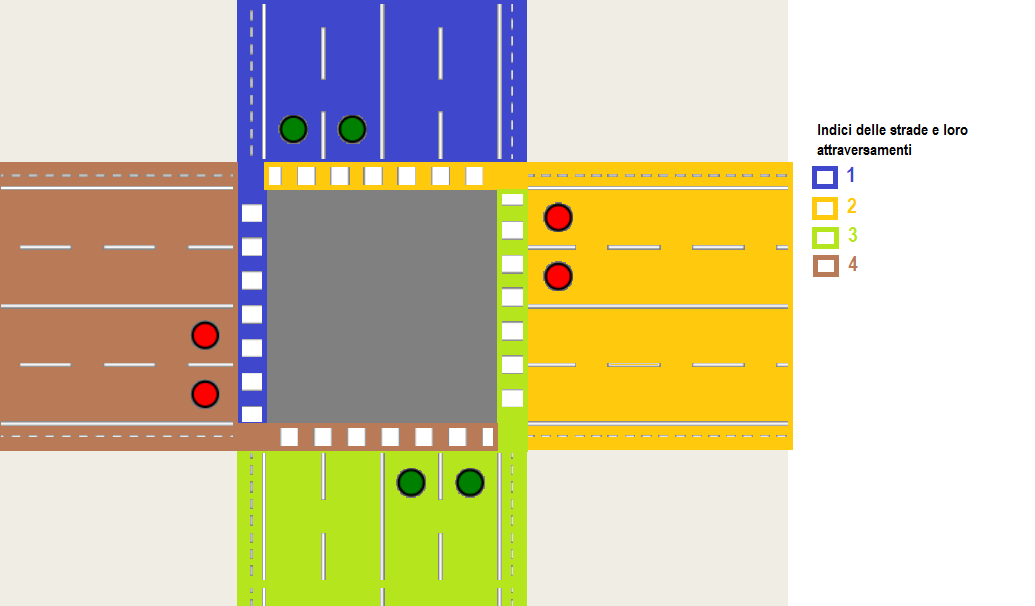
\includegraphics[width=1.0\linewidth]{IndexIncroci}}
\caption{Indici delle strade di un incrocio e relativi attraversamenti}
\label{fig:Indici delle strade di un incrocio e relativi attraversamenti}
\end{figure}

l'ordine scelto per lo spostamento delle entità prevede lo spostamento di veicoli, bici e pedoni; di seguito vengono riportate con delle figure le traiettorie che un task di tipo incrocio ha la responsabilità di gestione:

\begin{figure}[H] % Example image
\center{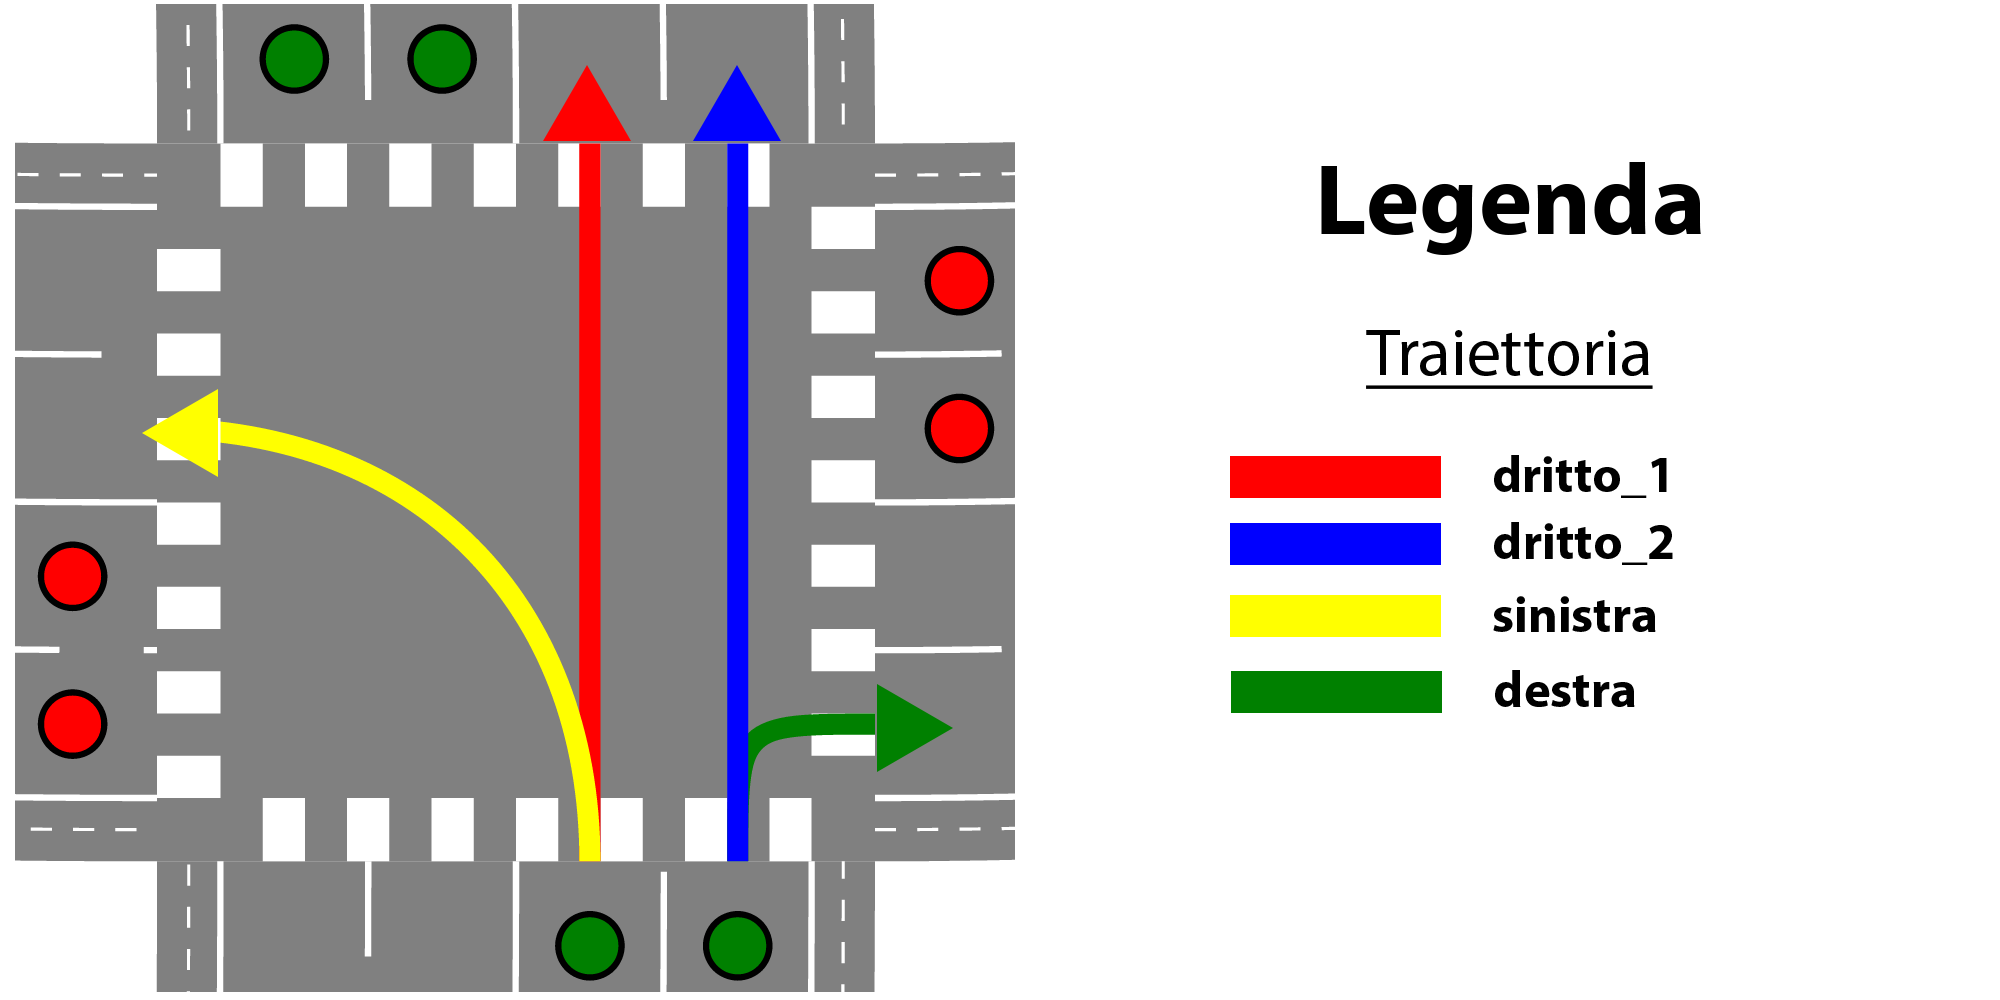
\includegraphics[width=1.0\linewidth]{traiettorie_incrocio_auto}}
\caption{Traiettorie per lo spostamento dei veicoli provenienti da una strada principale.}
\label{fig:Traiettorie per lo spostamento dei veicoli provenienti da una strada principale}
\end{figure}

\begin{figure}[H] % Example image
\center{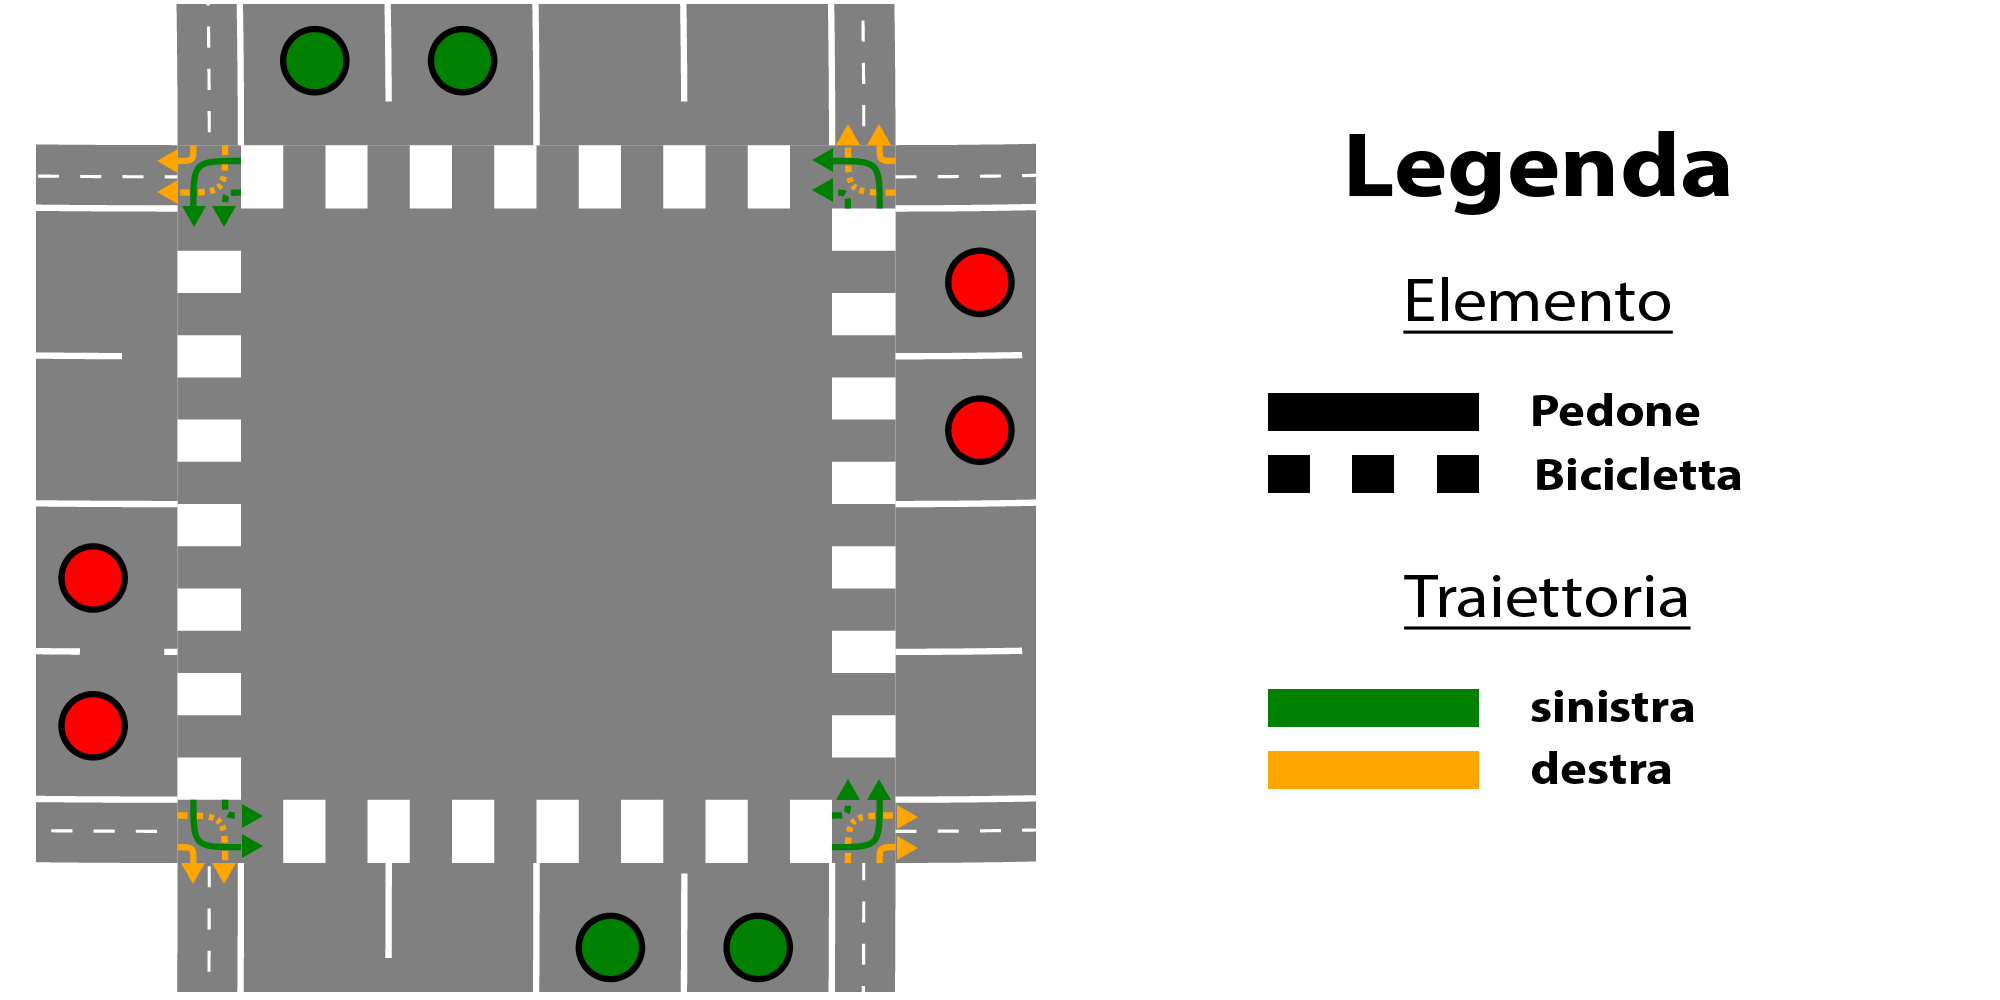
\includegraphics[width=1.0\linewidth]{traiettorie_incrocio_pedoni}}
\caption{Traiettorie per lo spostamento di bici/pedoni.}
\label{fig:Traiettorie per lo spostamento di bici/pedoni provenienti da una strada principale}
\end{figure}

I passi svolti dal task per effetture lo spostamento delle entità passive sono i seguenti:
\begin{enumerate}
\item l'entità attiva deve gestire lo spostamento dei veicoli provenienti da ogni strada, in tutte le traiettorie che un veicolo può impegnare nell'incrocio, quindi dovranno essere eseguiti i seguenti passi:
\begin{enumerate}
\item si prenda uno dei veicoli che l'entità deve spostare, (V\_A);
\item se il veicolo si trova completamente, in toto alla sua lunghezza, nella traiettoria dell'incrocio in cui deve essere spostato allora deve essere notificata la strada principale da cui proveniva V\_A del fatto che l'entità è stata interamente spostata nell'incrocio;
\item deve essere eseguito il calcolo della distanza da V\_A al veicolo successivo e tale calcolo dipende dal tipo di traiettoria che il veicolo deve attraversare, per semplicità di esposizione viene esposto il calcolo che deve essere eseguito da parte di un'entità proveniente dalla strada principale numero 3, vedi figura \ref{fig:Indici delle strade di un incrocio e relativi attraversamenti}:
\begin{itemize}
\item se il veicolo si trova in posizione 0 rispetto alla traiettoria che deve percorrere, allora occorre controllare se il semaforo per la traiettoria che il veicolo deve percorrere è verde o rosso. Se il semaforo è verde l'entità che intende attraversare deve controllare se esistono delle bici/pedoni in attraversamento dalla strada principale 4 (se esiste) in traiettoria \textit{drit\-to\_bi\-ci, drit\-to\_pe\-do\-ni} e fintanto che esistono delle entità in spostamento su queste traiettorie, V\_A non potrà avanzare; eseguito questo controllo si deve considerare lo stato di avanzamento delle macchine provenienti dalla strada principale 4: in particolare se esistono dei veicoli (V\_B) che dalla strada 4 percorrono le traiettorie \textit{dritto\_1 o dritto\_2}, V\_A dovrà fermarsi se si avrà che un qualunque veicolo V\_B interseca parte della traiettoria di V\_A; altrimenti se V\_B è in percorrenza la traiettoria di tipo \textit{sinistra}, allora se V\_A sta percorrendo la traiettoria \textit{dritto\_2 o destra} allora V\_B non è compromettente per le traiettorie di V\_A altrimenti se V\_A è in percorrenza la traiettoria \textit{sinistra} allora V\_A dovrà fermarsi fintanto che V\_B non abbia superato in toto l'intersezione della traiettoria di \textit{sinistra} di V\_B con quella di \textit{sinistra} di V\_A; mentre se V\_A percorre la traiettoria \textit{dritto\_1} allora dovrà fermarsi fintanto che V\_B non abbia completato la traiettoria \textit{sinistra}; se i controlli precedenti sono terminati con successo occorre controllare lo stato di avanzamento delle entità nella strada 2 (se esiste), da notare che questa strada come la strada 4 analizzata in precedenza presenterà semaforo rosso; se l'entità V\_A deve percorrere traiettorie \textit{dritto\_1, dritto\_2 e sinistra} e le entità V\_B sono in percorrenza le traiettorie \textit{dritto\_1 e dritto\_2} uscenti dalla strada 2, allora V\_A dovrà fermarsi fintanto che esista una traiettoria V\_B  che inersechi le traiettorie di V\_A (se V\_A deve percorrere la traiettoria sinistra allora si dovrà fermare finchè non esista alcuna entità V\_B in percorrenza la traiettoria \textit{dritto\_1}; se V\_A deve procedere per la traiettoria \textit{dritto\_2} e V\_B è in percorrenza la traiettoria \textit{destra} allora V\_A dovrà fermarsi; mentre se V\_B è in percorrenza la traiettoria \textit{sinistra} allora V\_A dovrà fermarsi fintanto che esista un veicolo V\_B che intersechi parte della traiettoria che V\_A deve percorrere;
\item allo step precedente sono stati eseguiti tutti i controlli necessari per iniziare l'avanzamento di un veicolo nel caso si trovi in posizione 0 con semaforo verde; quei controlli sono necessari al fine di permettere il completamento dell'attraversamento di quei veicoli o quei pedoni che avevano impegnato l'incrocio a semaforo verde ma che nel corso della gestione del loro spostamento è scattato il semaforo rosso, quindi la precondizione per iniziare lo spostamento di veicoli che presentano semaforo verde è di non muoversi fintanto che le loro traiettorie sono intersecate in qualche punto da veicoli le cui strade di provenienza hanno semaforo rosso; il protocollo poi a controlli validati inizia (se V\_A si trova in posizione 0 nella sua traiettoria) o continua lo spostamento di un'entità V\_A (se per essa è già stato gestito uno spostamento);
\item se il veicolo V\_A deve impegnare la traiettoria \textit{destra}, allora dovrà calcolare la posizione dalla prossima entità che la sua traiettoria incontra; se non vi sono entità situate ad una distanza maggiore nella medesima traiettoria allora dovrà essere calcolata la distanza con la prima entità che V\_A incontrerà nella corsia della strada principale destinazione di V\_A quindi della strada 2; se la prossima entità incontrata è un'entità presente nella strada di destinazione di V\_A allora è necessario fissare un limite alla distanza in modo tale da garantire che, grazie alla distanza limite fissata, il veicolo V\_A non aggiorni la sua posizione con una posizione compromettente per le decisioni di avanzamento prese dall'entità della strada principale, dato che questa inizierà la gestione per l'entità V\_A solo dal quanto di sistema successivo (questa limitazione è fissata per ogni tipologia di traiettoria gestita dall'incrocio); V\_A inoltre se procede nella traiettoria \textit{destra} dovrà, prima di completare l'avanzamento, dare la precedenza a quelle bici/pedoni in attraversamento la traiettoria \textit{drit\-to\_bi\-ci e drit\-to\_pe\-do\-ni} dalla strada principale 3, vedi figura \ref{fig:Indici delle strade di un incrocio e relativi attraversamenti};
\item se il veicolo V\_A deve impegnare la traiettoria \textit{dritto\_1 o dritto\_2}, analogamente al sistema descritto al punto precedente, deve essere calcolata la distanza dal prossimo veicolo e dovrà essere data la precedenza a quelle eventuali (bici/pedoni) in attraversamento la traiettoria \textit{drit\-to\_bi\-ci e drit\-to\_pe\-do\-ni} dalla strada principale 2; i veicoli percorrenti la traiettoria in descrizione hanno la precedenza su quei veicoli (V\_B) in percorrenza la traiettoria sinistra dalla strada principale 1 ed il veicolo V\_B darà la precedenza ai veicoli percorrenti le traiettorie in descrizione; quindi V\_A nel caso in cui esista un veicolo V\_B che copre una posizione minore a quella per cui deve dare la precedenza allora V\_A la otterrà di certo, altrimenti (se V\_B si trova ad una posizione che ha superato il limite entro il quale dare la precedenza, e tale limite poteva essere superato dato che non esisteva alcun veicolo a cui spettava la precedenza) sarà V\_A ad attendere che V\_B sia uscito dalla zona di intersezione con la traiettoria di V\_A;
\item se il veicolo V\_A deve percorrere la traiettoria \textit{sinistra}, allora deve essere calcolata analogamente ai punti precedenti la distanza con la prossima entità che V\_A incontra ed eventualmente dovrà essere data la precedenza a quelle entità (bici/pedoni) in attraversamento la traiettoria \textit{drit\-to\_bi\-ci e drit\-to\_pe\-do\-ni} dalla strada principale 3, vedi attraversamento della strada 3 in \ref{fig:Indici delle strade di un incrocio e relativi attraversamenti}; inoltre V\_A deve dare la precedenza prima a veicoli V\_B percorrenti la traiettoria dritto\_1 e poi a quei veicoli V\_B percorrenti la traiettoria dritto\_2.
\end{itemize}
\item se il veicolo (V\_A) ha completato l'attraversamento della traiettoria, allora può essere eseguita la configurazione delle proprietà del veicolo al fine che questo possa essere gestito correttamente dall'entità della strada principale di destinazione; il task in esame dovrà interrogare il servizio di locazione delle entità al fine di apprendere la configurazione del percorso di V\_A e quindi la configurazione da dare a V\_A stesso, infine potrà essere inserito il veicolo nella mailbox della strada principale di destinazione che, visto il protocollo della strada principale, che provvederà alla gestione del veicolo V\_A a partire dal quanto di sistema successivo.
\end{enumerate}
\item l'entità attiva, per gestire lo spostamento di bici/pedoni, dovrà eseguire l'avanzamento delle entità su ogni attraversamento pedonale dell'incrocio; l'incrocio prevede sempre 4 attraversamenti pedonali indipendentemente dal fatto che l'incrocio sia un incrocio con 3 o con 4 strade, per esempio se si considera un incrocio con 3 strade in cui la strada mancante è la 2, gli attraversamenti pedonali in direzione \textit{dritto\_1 e dritto\_2} dalla strada 2 verranno utilizzati per permettere le svolte in direzione \textit{sinistra} da parte di (bici/pedoni); di seguito i passi del protocollo per gestire lo spostamente di bici/pedoni negli incroci:
\begin{enumerate}
\item lo spostamento di (bici/pedoni) deve essere eseguito per ogni attraversamento pedonale dell'incrocio, per semplificare la spiegazione del protocollo si considera lo spostamento per l'attraversamento pedonale relativo alla strada principale 3 dell'incrocio; le traiettorie su cui effettivamente un'entità (bici/pedone) può essere spostata sono \textit{des\-tra\_bi\-ci, des\-tra\_pe\-do\-ni, drit\-to\_bi\-ci, drit\-to\_pe\-do\-ni}, quindi le entità che devono seguire la traiettoria di \textit{sinistra} dovranno spostarsi per 2 attraversamenti pedonali in cui su entrambi seguiranno la traiettoria di \textit{drit\-to\_bi\-ci o drit\-to\_pe\-do\-ni};
\item un'entità (V\_B) che proviene dall'attraversamento pedonale perpendicolare a quello relativo alla strada 3, ovvero l'attraversamento pedonale della strada 4, (vedi \ref{fig:Indici delle strade di un incrocio e relativi attraversamenti}) può voler proseguire in direzione dritto e quindi immettersi nella strada 2 o svoltare a sinistra e quindi percorrere, in entrambi i casi, la traiettoria \textit{drit\-to\_bi\-ci o drit\-to\_pe\-do\-ni} appartenenti all'attraversamento pedonale della strada 3; se V\_A proveniente dalla strada 4 vuole proseguire in direzione dritto verso la strada 2, è necessario inserire pedoni e bici nella traiettoria \textit{des\-tra\_bi\-ci o des\-tra\_pe\-do\-ni} della strada 3, al fine di permettere alle entità provenienti dall'attraversamento della strada 4 di liberare l'attraversamento il più in fretta possibile evitando obblighi di precedenza di questi nei confronti di entità su traiettorie perpendicolari; quindi se non vi sono entità da spostare nella traiettorie \textit{des\-tra\_bi\-ci o des\-tra\_pe\-do\-ni} si deve controllare se ci sono delle entità in attraversamento dalla strada 4, che vogliono muoversi verso la strada 2 e quindi inserirle nelle traiettorie \textit{des\-tra\_bi\-ci o des\-tra\_pe\-do\-ni}; l'inserimento di queste entità nelle traiettorie appena dette, potrà essere effettuato solo se nella strada 3 esiste spazio sufficiente per accomodarle al fine di evitare sovrapposizioni di entità nei marciapiedi/piste ciclabili. Lo spostamento poi dell'entità (V\_A) inserita nella traiettoria \textit{des\-tra\_bi\-ci o des\-tra\_pe\-do\-ni} può avvenire considerando la distanza con la prossima entità, presente nella traiettoria stessa o altrimenti ottenuta interrogando la mailbox della strada principale di destinazione di V\_A; in questo caso quindi l'attraversamento può avvenire anche se esistono delle entità, presenti nelle traiettorie drit\-to\_bi\-ci e drit\-to\_pe\-do\-ni della strada 3 o della strada 4, che intersecano delle entità in attraversamento nelle traiettorie in descrizione;
\item l'altra tipologia di traiettoria che pedoni/bici possono percorrere nell'incrocio sono \textit{drit\-to\_bi\-ci o drit\-to\_pe\-do\-ni}; le entità che possono appartenere a questa traiettoria sono quelle provenienti dalla strada 3, che intendono procedere in direzione dritto o sinistra, oppure quelle entità provenienti dall'attraversamento della strada 4 che intendono percorrere la direzione sinistra;\\
se ci sono delle entità (V\_A) che si trovano in posizione 0 nella traiettoria \textit{drit\-to\_bi\-ci o drit\-to\_pe\-do\-ni} o se esistono delle entità che sono in attesa di essere spostate nelle traiettorie appena dette perchè provenienti dalla strada 4 con direzione sinistra allora si deve controllare dapprima se il semaforo per queste entità è verde; se il semaforo è verde e non esiste già un'entità (bici/pedone) in attraversamento nelle traiettorie in descrizione in una posizione tale per cui ogni altro veicolo gli darà la precedenza allora sono necessari i seguenti controlli: si controlla se esistono dei veicoli (V\_B) provenienti dalla strada 3 in svolta a destra, in tal caso l'entità V\_A dovrà fermarsi in posizione 0 fintanto che il veicolo V\_B non ha completato l'attraversamento nella traiettoria \textit{destra}; occorre poi controllare se esiste un qualche veicolo V\_B proveniente dalla strada 4 in direzione \textit{dritto\_1 o dritto\_2}, affinchè V\_A possa iniziare l'attraversamento, in modo tale da permettere ai veicoli V\_B di completare l'attraversamento dato che questi provengono da una strada con semaforo rosso nel quanto di sistema in corso; quindi si deve controllare se esitono dei veicoli provenienti dalla strada 1 in percorrenza la traiettoria sinistra e infine se esistono dei veicoli in uscita dalla strada 2, tale che intersechino l'attraversamento pedonale della strada 3; quindi se questi controlli sono andati a buon fine V\_A può impegnare l'incrocio e avrà la precedenza su qualsiasi altro veicolo che impegnerà l'incrocio; nel caso in cui esisteva già un'entità (bici/pedone) che aveva impegnato l'incrocio i controlli qui riportati possono essere saltati dato che i veicoli daranno sempre la precedenza a quelle bici/pedoni che hanno già impegnato l'incrocio; con un esempio se un veicolo si trova su una certa traiettoria, verrà controllato se esistono delle bici/pedoni su cui occorre dare la precedenza a patto che questi abbiano già impegnato l'incrocio, mentre se le bici/pedoni si trovano in posizione 0, significa che non hanno impegnato l'incrocio e quindi i veicoli potranno completare l'attraversamento della traiettoria sapendo che i pedoni/bici daranno ai veicoli la precedenza dato che questi ultimi hanno già impegnato l'incrocio; \\
a questo punto se non esiste alcuna entità V\_A appartenente alla traiettoria \textit{drit\-to\_bi\-ci o drit\-to\_pe\-do\-ni} in una posizione che interseca parte della strada principale, è possibile inserire le entità che provengono dalla strada 4 e che devono seguire la direzione sinistra, nelle traiettorie in descrizione purchè nella strada principale 3 esista spazio sufficiente per accomodare le entità da spostare nelle traiettorie \textit{drit\-to\_bi\-ci o drit\-to\_pe\-do\-ni}; \\
per le entità (bici/pedoni) che hanno già impegnato gli attraversamenti o per quelle entità situate in posizione 0 e che al punto precedente hanno ottenuto l'abilitazione per l'attraversamento è possibile eseguire l'avanzamento (come per tutte le entità, se un'entità ha impegnato l'incrocio allora, indipendentemente dal colore del semaforo da cui l'entità proveniva, deve essere completato l'avanzamento); \\
l'avanzamento per un'entità (V\_A) appartenente alle traiettorie \textit{drit\-to\_bi\-ci o drit\-to\_pe\-do\-ni} deve avvenire considerando la distanza rispetto all'entità successiva nella medesima traiettoria e considerando l'effettiva destinazione per un'entità V\_A:
\begin{itemize}
\item se V\_A (proveniente dalla strada 3) deve procedere verso la strada 1, in direzione dritto quindi, allora V\_A dovrà percorrere completamente la traiettoria e considerare poi la distanza dalla prima entità presente nella strada 1 solamente se non esiste la strada 2; infatti se esiste la strada 2 allora V\_A, in base a ciò che è stato detto nei punti precedenti, dovrà essere inserito nelle traiettorie \textit{des\-tra\_bi\-ci o des\-tra\_pe\-do\-ni} e quindi la traiettoria di V\_A dovrà essere percorsa solamente fintanto che V\_A sia completamente uscito dalla parte di attraversamento che interseca la strada principale su cui l'attraversamento è situato; la situazione è analoga per quell'entità V\_A che deve procedere nella direzione di sinistra; in base alla destinazione quindi di V\_A e alla configurazione della mappa nell'incrocio gestito dal task in esame si dovrà procedere con l'inserimento di V\_A o in una struttura temporanea per quell'entità (cioè una struttura che verrà utilizzata per accogliere le entità che devono procedere in direzione sinistra, o in direzione dritto nel caso in cui esista la strada 2) al fine di permettere l'inserimento di V\_A (nei prossimi quanti di sistema) nelle traiettorie giuste per completare l'attraversamento dell'incrocio; altrimenti, se le condizioni precedenti non si verificano (in particolare la strada 2 non esiste), V\_A dovrà essere inserito nella mailbox della strada principale di destinazione di V\_A, quindi sulla mailbox della strada 1.
\end{itemize}
\end{enumerate}
\end{enumerate}

\subsubsection*{Operazioni dopo la nuova sincronizzazione} 
Il task gestore degli incroci dopo aver effettuato l'operazione di sincronizzazione, potrà rendere effettivi gli aggiornamenti di posizione delle entità calcolati nel quanto di sistema precedente; l'operazione di aggiornamento per entità di tipo veicolo gestite da un'entità di tipo incrocio consiste semplicemente nel rendere effettivi gli aggiornamenti di posizione calcolati al quanto precedente. Mentre per gli spostamenti di bici/pedoni è necessario eseguire anche lo spostamento delle entità da una determinata traiettoria ad un'altra nel caso siano soddisfatte le condizioni di spostamento esaminate nel protocollo. Quindi qui potrà essere notificata la view della nuova posizione delle entità che occupano alla fine del quanto di sistema precedente.  